\chapter{Problem analysis}

This chapter provides details on the problem the application is trying to solve and describes user requirements which specify what functionality the application should provide to its users. It also includes an overview of existing solutions for the connection search problem. Finally, it describes the available data necessary to provide the functionality and its structure.

\section{Problem description}

In this section, we will first introduce the problem's domain and explain all the necessary terms we will be using later. Then we will describe the core of the problem our application is trying to solve.

\subsection{Domain introduction}

\begin{figure}[h!]
    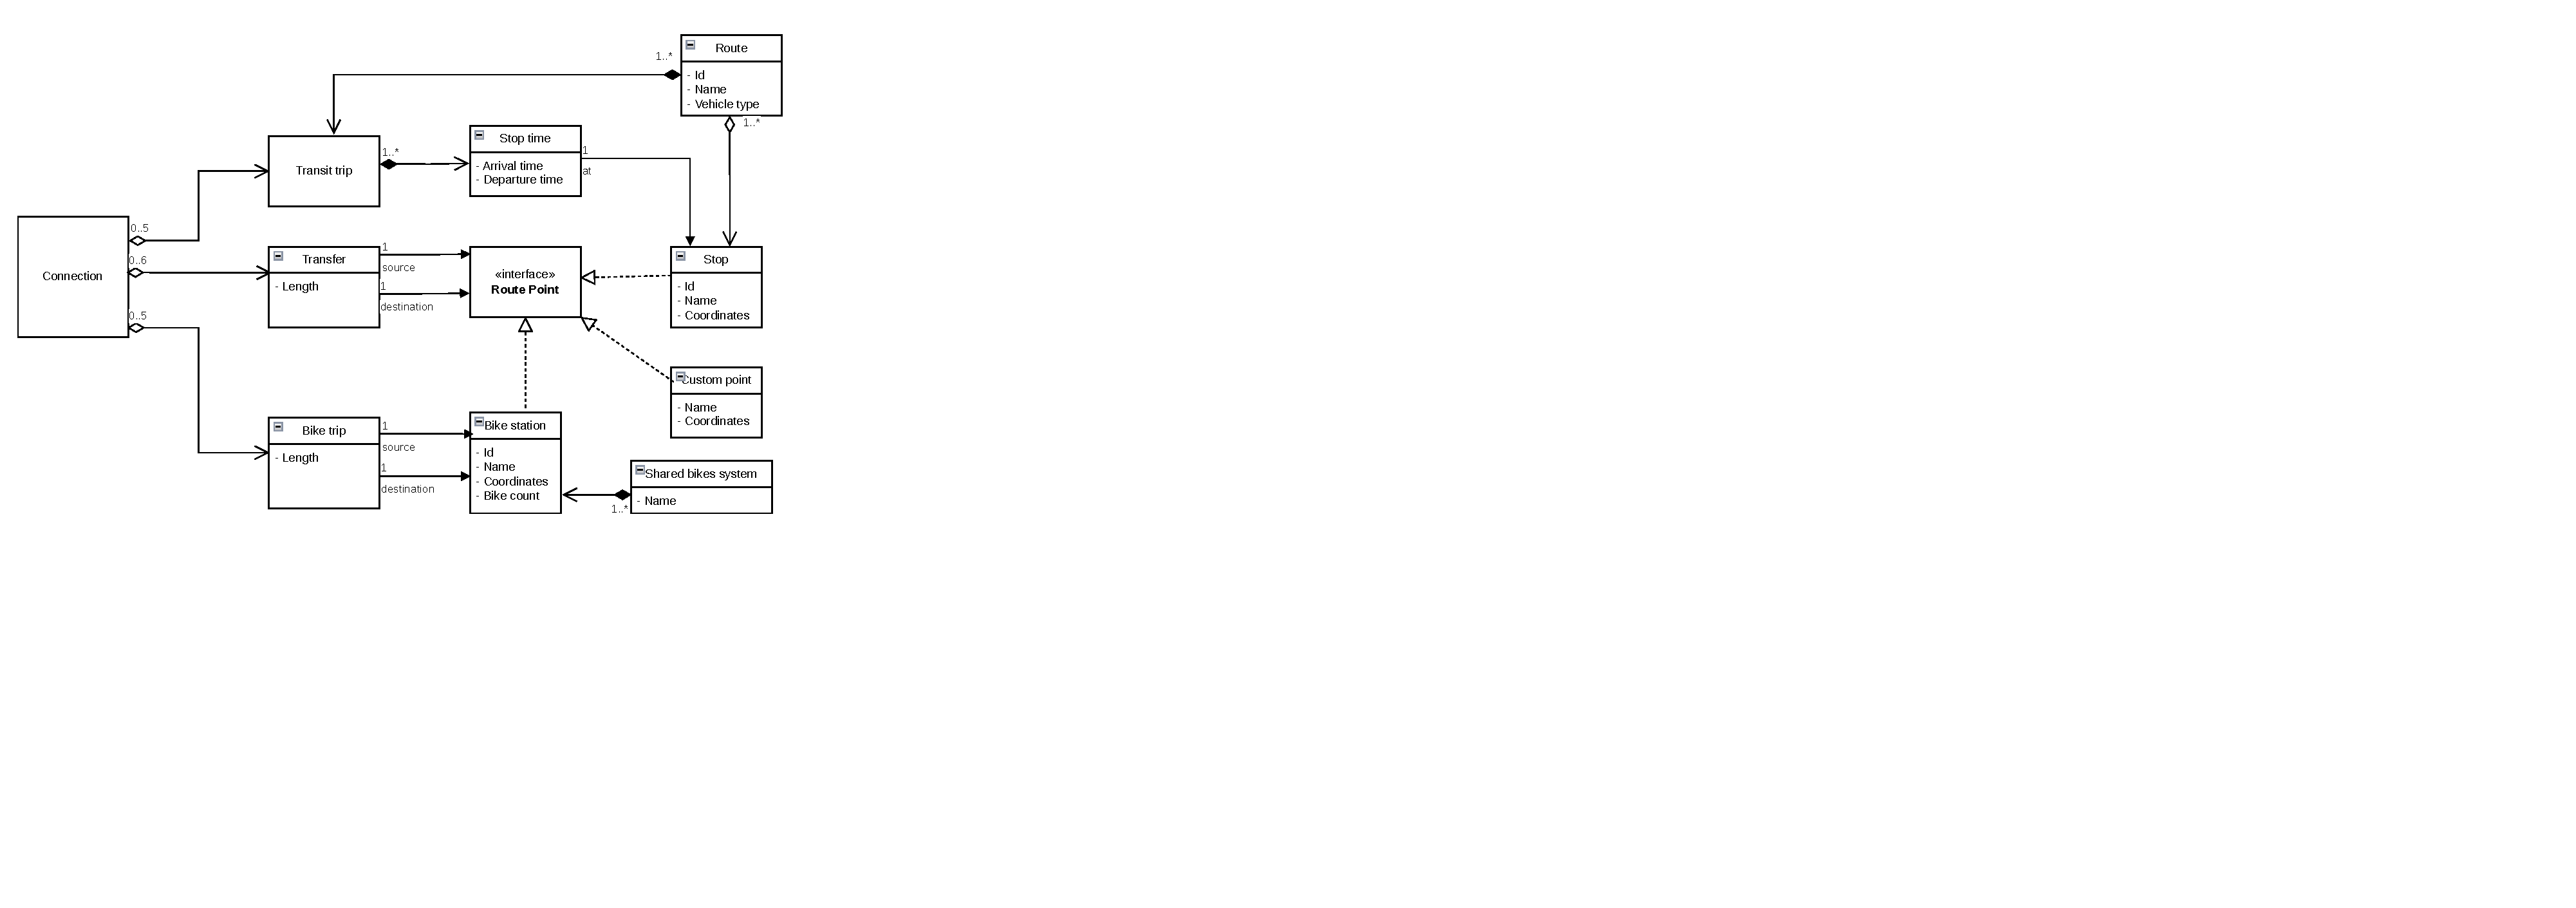
\includegraphics[width=\textwidth]{img/domain_model.pdf}
    \caption{The domain model}
    \label{fig:domain_model}
\end{figure}

The resulting object we want to produce and show to the user is a \texttt{Connection}. A \texttt{Connection} is a list consisting of public transit \texttt{Trips}, \texttt{Transfers} and \texttt{Bike trips}. 

Every \texttt{Trip} serves one \texttt{Route}. A \texttt{Route} consists of a list of \texttt{Stops} and typically corresponds to what is usually known as a line. It has an id, name and a vehicle type describing what vehicle the \texttt{Route} is being served by (i.e. Bus/Tram/Metro/...). However, it is important to note that the relationship between a \texttt{Route} within the context of our application and a real-world line is not always 1:1. Typically, one line will have multiple different variations (shorter variations, variations with vehicles pulling in and out of the depots, variations where not all stops are served, ...). All of these variations will share the same line name, however, each of them is a separate \texttt{Route} with its separate list of \texttt{Stops}.

A \texttt{Trip} consists of a list of \texttt{Stop Times}. A \texttt{Stop Time} specifies both the arrival and departure times of the \texttt{Trip} at the corresponding \texttt{Stop} of the \texttt{Trip}'s \texttt{Route}.

A \texttt{Transfer} represents travel on foot. It consists of two points - the source and the destination \texttt{Route Points}. A \texttt{Route Point} can be either a \texttt{Stop}, a \texttt{Bike Station} or a \texttt{Custom point}.

A \texttt{Stop} represents a single point within the public transit network where it is possible to board or disembark public transit \texttt{Trips}. It is important to mention that a \texttt{Stop} within the context of our application does not directly correspond to what most people imagine under the term. Typically, a "stop" is described by its name, i.e. all boarding points sharing the same name are considered a single "stop". In our context, every single one of these boarding points is its own separate \texttt{Stop}. Within Prague's public transit network, this typically means that each \texttt{Stop} corresponds to a separate stop sign. The set of \texttt{Stops} sharing the same name is called a \texttt{Node}.

A \texttt{Custom point} is an arbitrary point within the connection, specified by its coordinates. Typically, it will be used to provide the user with the opportunity to set the source or target of his search to a specific coordinate point, instead of having to always select a specific \texttt{Stop}.

Finally, a \texttt{Bike Trip} represents travel on a shared bicycle. It consists of a source and destination \texttt{Bike Station}. A \texttt{Bike Station} is a single point within a particular \texttt{Bikesharing system} at which it is possible to borrow and return bicycles. Every \texttt{Bikesharing System} has its own set of \texttt{Bike Stations}, each of which is specified by an id, name and coordinates and has a certain number of currently available bicycles in it. A \texttt{Bike Trip} cannot be performed between \texttt{Bike Stations} that belong to different \texttt{Bikesharing Systems}.

To collectively describe the three different parts of a \texttt{Connection} (\texttt{Trips}, \texttt{Transfers} and \texttt{Bike Trips}, we will use the term \texttt{Segments}.


\subsection{Core problem definition}

The core problem the application is trying to solve is the connection search problem. The user needs to be able to use the app to search for efficient connections between two points within Prague's public transit network that they specify. Furthermore, to account for both use cases where the user wants to depart after a certain time and where they want to arrive before a certain time, the application will need to be able to handle both of these options. The application needs to be able to find and show this resulting connection (or multiple alternative connections) to the user.

As stated above, each connection will consist of trips, transfers and bike trips. Between any 2 consecutive trips within a connection, there may be any number of transfers or bike trips. This means that if the connection contains two or more public transit trips, for any 2 consecutive trips within the connection, the sum of durations of the transfers and bike trips between them needs to be less than or equal to the length of the time frame between the first trip's disembark time and the second trip's boarding time.

Furthermore, it is not allowed for two transfers to follow immediately after one another. The same is true for bike trips. This is to prevent the chaining of transfers or bike trips, which would render it useless to set a maximum time or distance for them. It is theoretically possible for 2 trips to follow directly after one another as the first one may arrive at the same exact stop as the second one departs, but for simplicity's sake, we will require a 0 meter long transfer to be inserted in between them in such situations. As it is not possible for bike trips to begin or end in public transit stops, this implies that within the list of trips, transfers and bike trips that a connection consists of, two segments of the same time may never occur directly consecutively.

Apart from the inclusion of bikesharing, this is the core functionality that any connection planning application must provide. The main goal of our application is to expand the functionality to provide more useful personalization options. These additional problems, features and solutions will be described in following chapters.

\section{Existing solutions}

As stated above, the goal of this application is to provide people living and working in Prague with a practical way to search for connections within Prague's extensive public transit network. However, there already exist many existing solutions serving the purpose of searching for public transit connections, so why is it necessary to develop another one? To answer this question, we will go over the existing solutions and describe their advantages and shortcomings. From this information, we will derive the requirements for our new, improved way to approach the problem.

The core functionality we explained in the previous chapter is identical for all existing solutions. For this reason, in this chapter we will only describe the functionality each of the solutions provides on top of this.

\subsection{Global solutions}

First of all, there are many solutions for public transit connection searching that promise to work worldwide and could thus also be used within Prague.

\subsubsection{Maps Google}
In addition to car and pedestrian routing, Google's Maps also provide routing between 2 points using public transportation. On top of the basics, they also include the option to prioritize certain transport modes and basic filtering options based on the user's comfort preference ("Best route", "Fewer transfers", "Less walking", "Wheelchair accessible"). However, the application also has many shortcomings for a regular public transit user. For instance, there is no way to adjust one's walking pace, search for the absolute fastest connections or to set the maximum distance of transfers and the app does not support bikesharing in its search. The app also does not properly support searching using stop names and uses local names and points of interest instead. Arguably the biggest drawback is the app's UI. While being practical for long-distance connections by providing an overview of general route options, it is very hard to compare the options and find the most suitable one, making this app impractical for short public transit connections within the city (\cref{fig:google_maps_1}). Furthermore, as there is no way to search for a connection without displaying the map, this application is also very data-intensive, which is not desired for a connection searching app.

\begin{figure}[h!]
    \begin{minipage}[b]{0.45\textwidth}
        \centering
        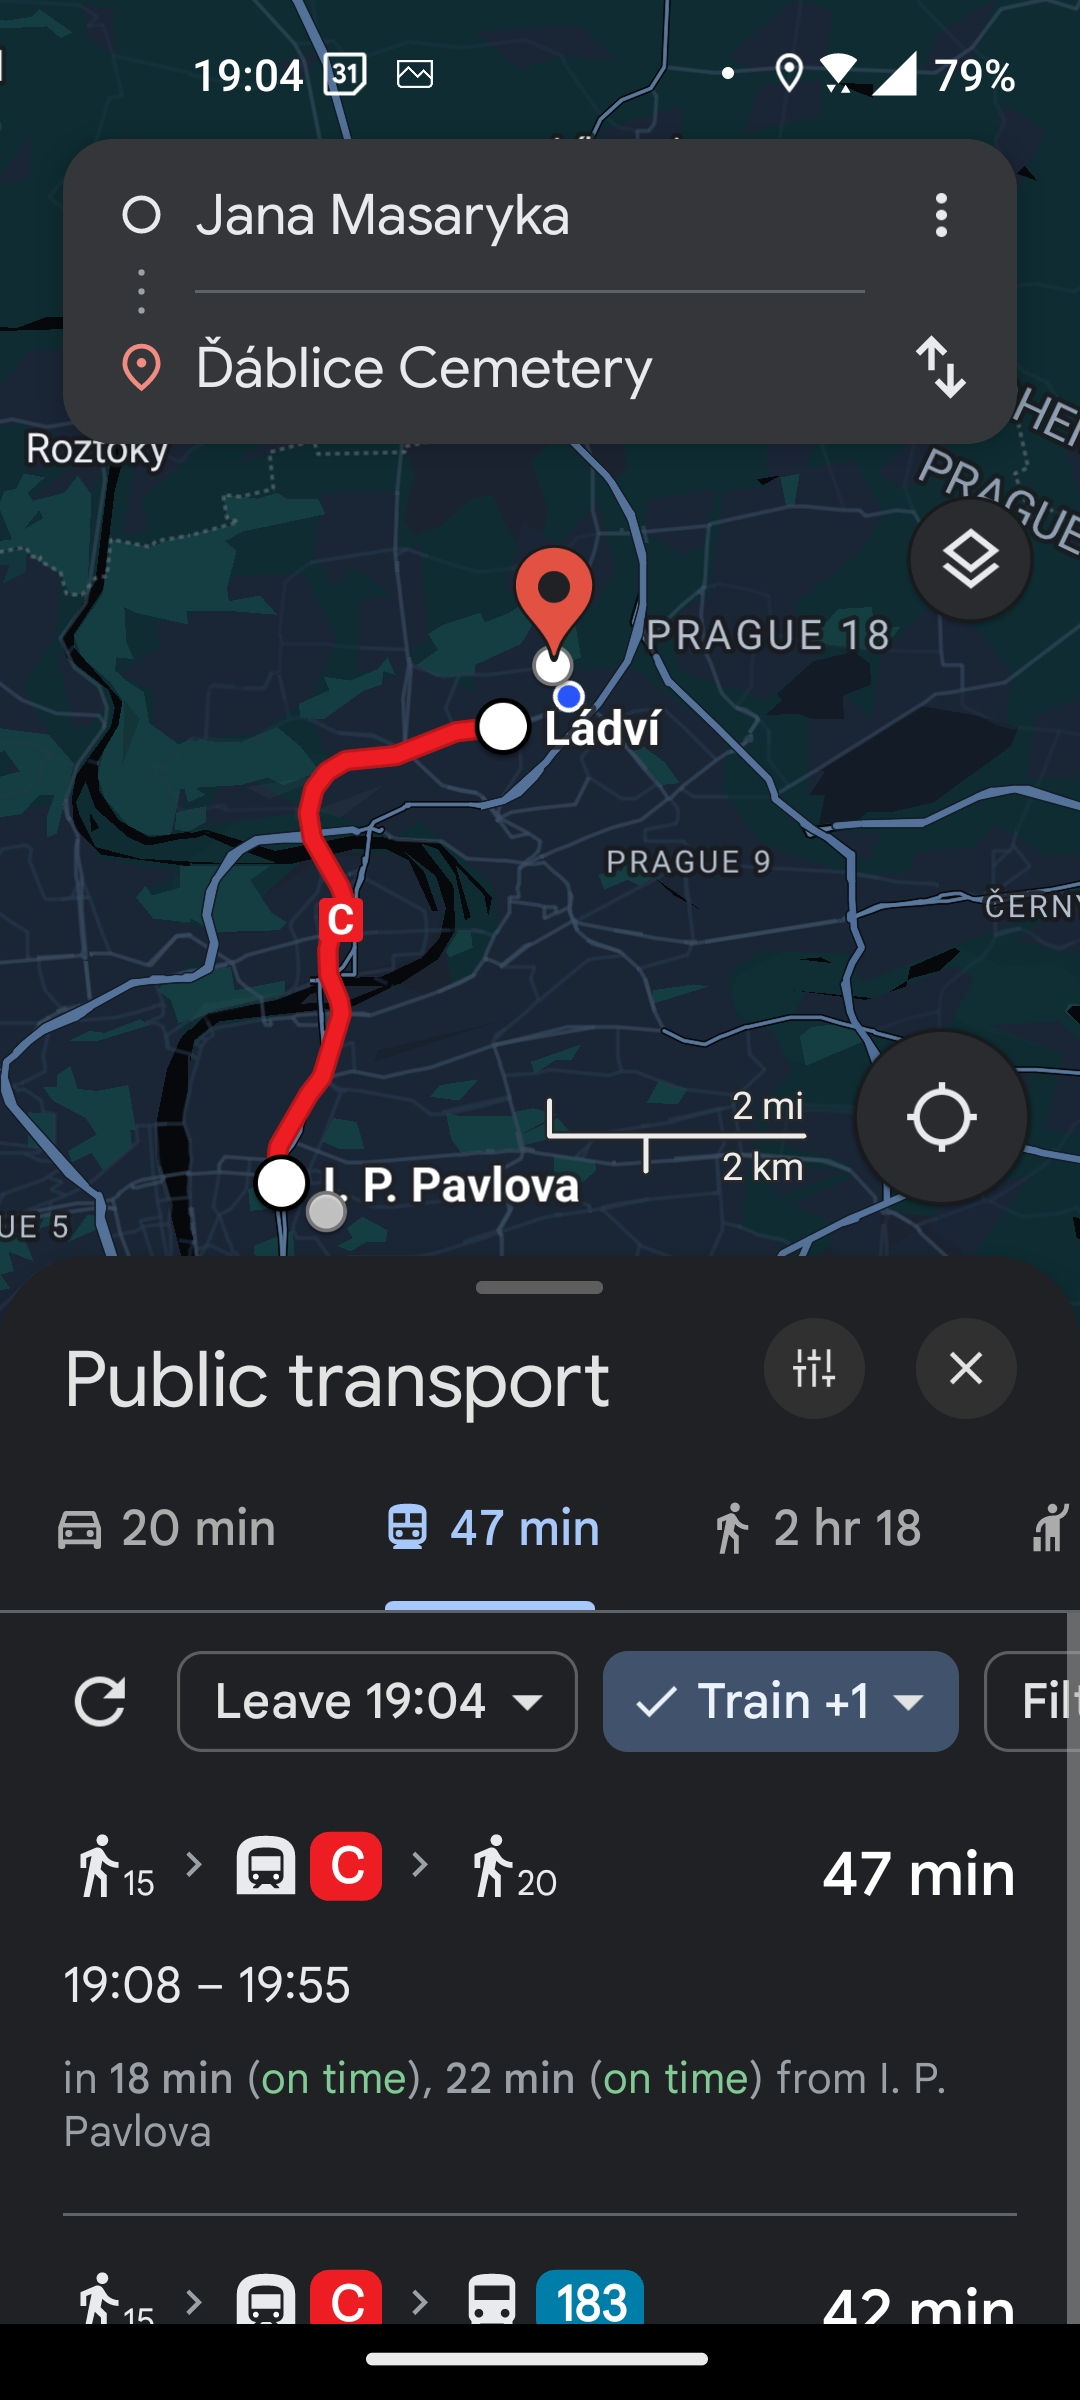
\includegraphics[width=\textwidth]{img/screenshots/google_maps_result_1.jpg}
    \end{minipage}
    \hfill
    \begin{minipage}[b]{0.45\textwidth}
        \centering
        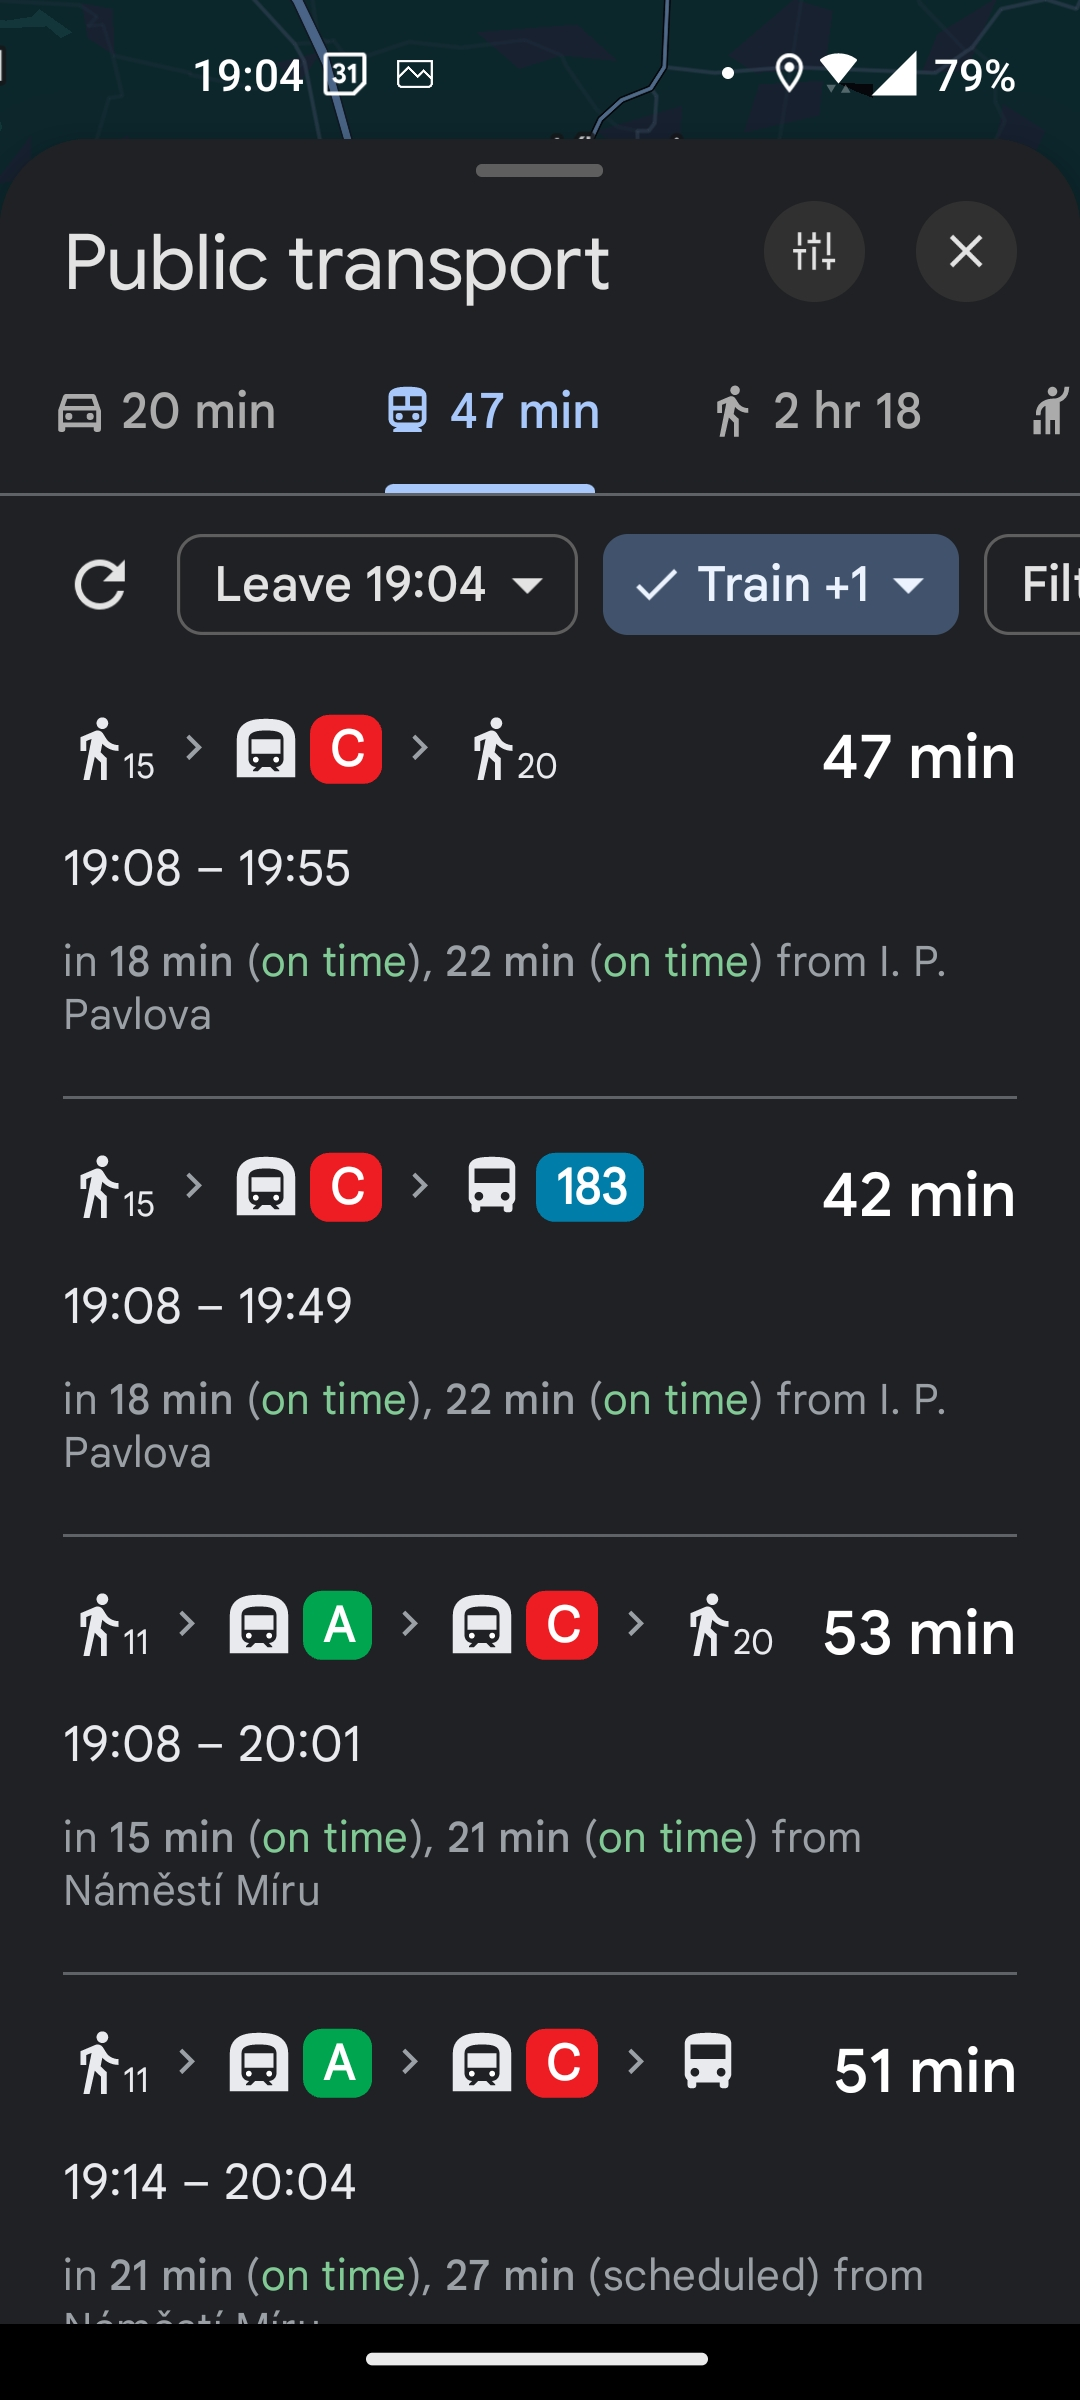
\includegraphics[width=\textwidth]{img/screenshots/google_maps_result_2.jpg}
    \end{minipage}
    \caption{Result of a connection search in Maps Google}
    \label{fig:google_maps_1}
\end{figure}

\subsubsection{Moovit}
Another option with global coverage is the Moovit app. Once again, there are some comfort preference setting options ("Best route", "Least walking", "Fewest transfers") and transit mode preference settings. This app also has an additional option for setting walking pace to slow, though there is no option for setting it to a specific value. The user can also set the maximum walk duration and search using stop names. However, the app also has many of the same issues as Google Maps, such as a distracting and confusing UI (\cref{fig:moovit}) and the lack of bikesharing support in Prague.



\begin{figure}[h!]
    \centering
    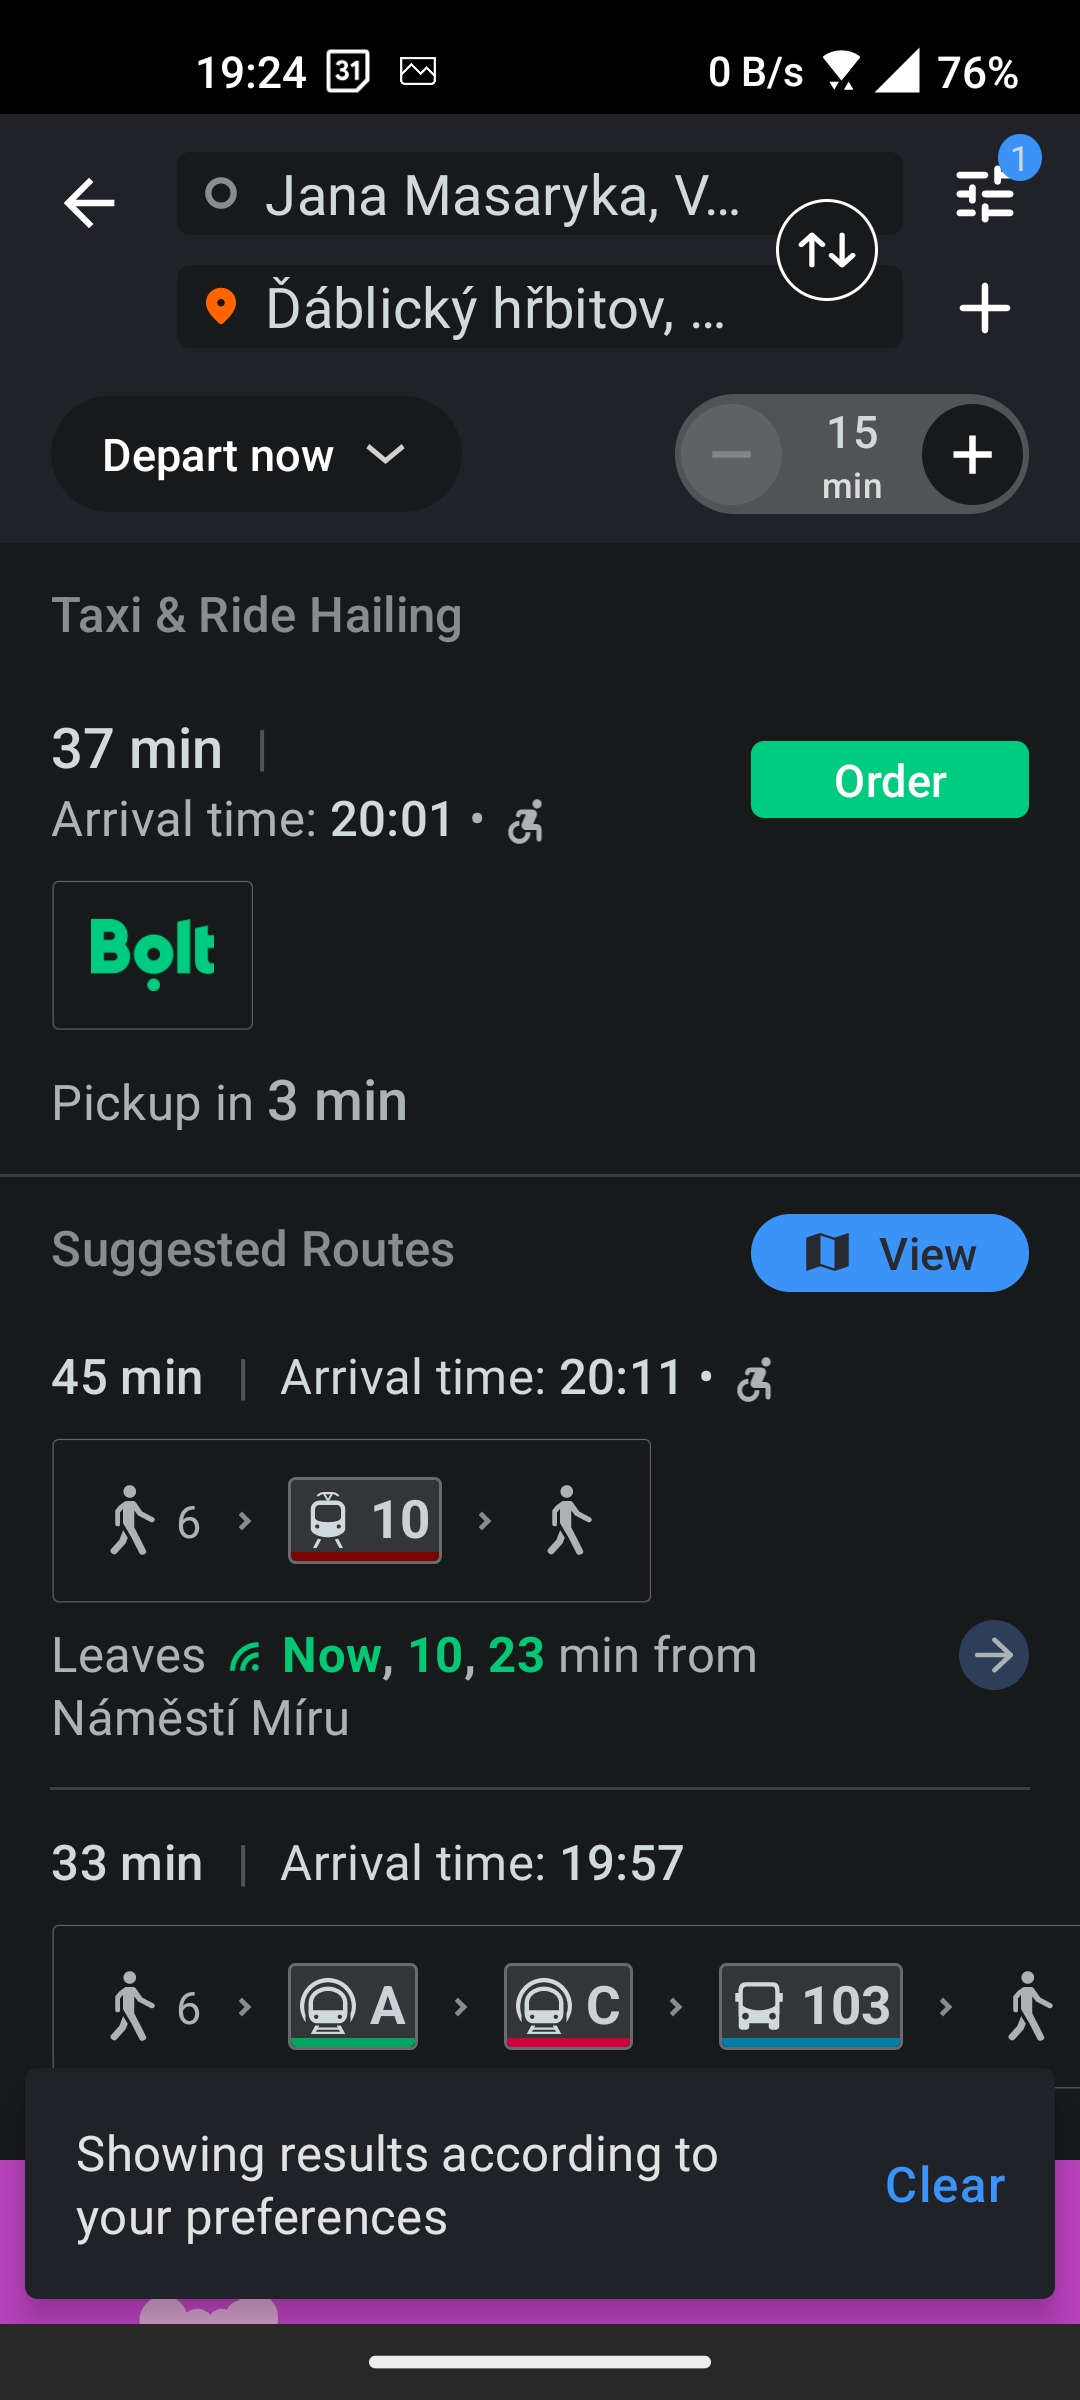
\includegraphics[width=0.45\textwidth]{img/screenshots/moovit_result.jpg}
    \caption{Result of a connection search in Moovit}
    \label{fig:moovit}
\end{figure}

\subsection{Country-wide solutions}

There also are some apps intended for the whole of Czech Republic, such as the following:

\subsubsection{IDOS}

IDOS is the most popular app for public transit connection searching in the Czech Republic. However, its search customization options are very limited. There are options for adding an intermediate stop, selecting transport modes and operators, only searching for direct connections, setting an absolute global transfer time and searching for wheelchair accessible connections. It lacks features such as comfort preference settings other than a direct connection search, setting maximum walking distance or walking pace or using bikesharing services. As opposed to many other apps, IDOS will also not consider connections starting from a different stop than the one entered by the user, even if it were a relatively short transfer and it would greatly reduce the arrival time. However, IDOS's UI is much more intuitive and practical for city-level public transit trips than those of the global apps, enabling the user to gain a better overview of their options through scrolling through all the available connections (\cref{fig:idos}).

\begin{figure}[h!]
    \centering
    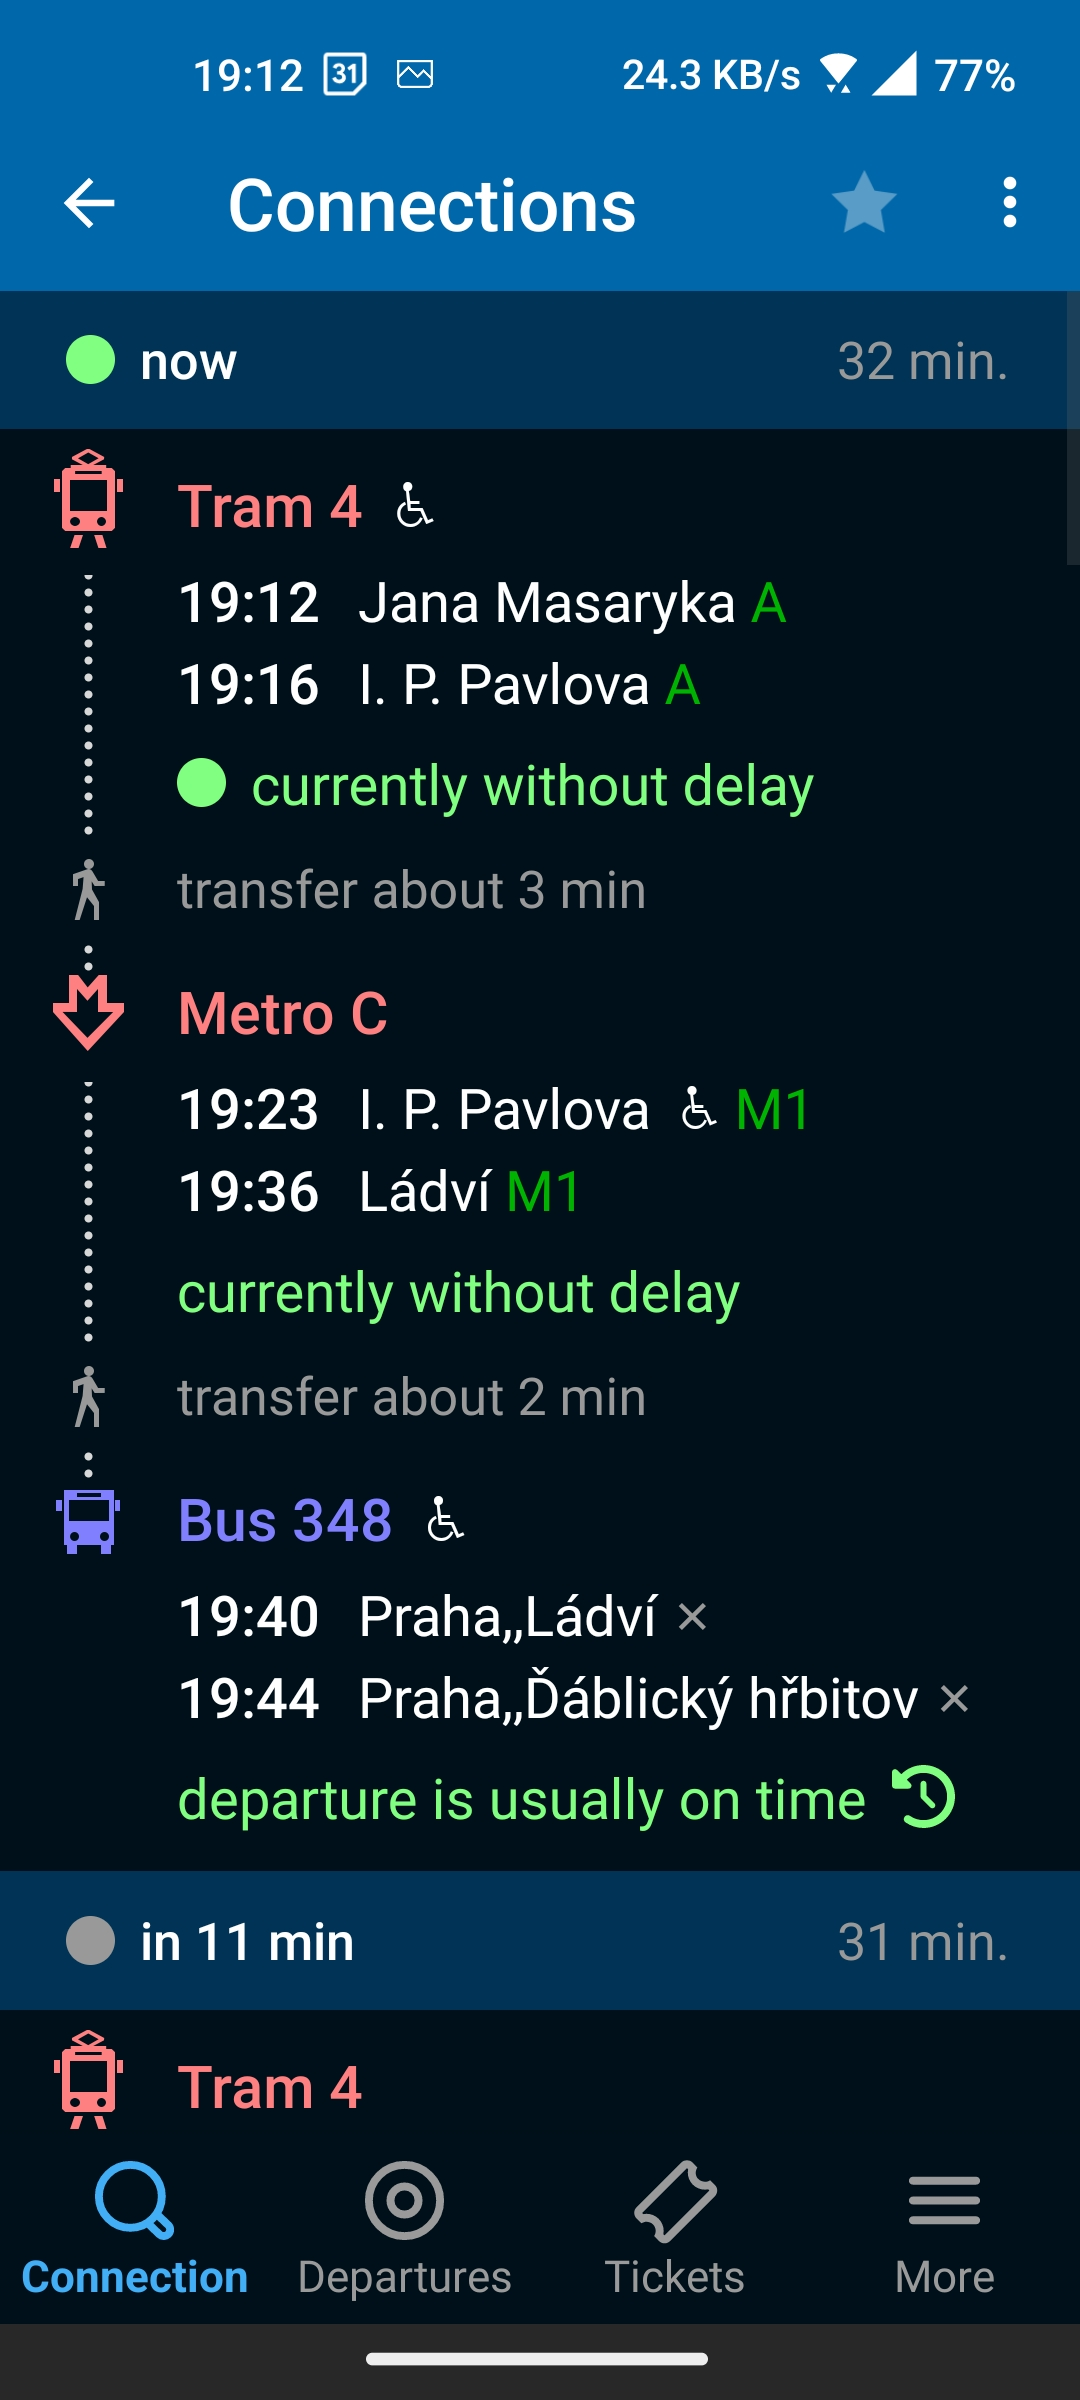
\includegraphics[width=0.45\textwidth]{img/screenshots/idos_result.jpg}
    \caption{Result of a connection search in IDOS}
    \label{fig:idos}
\end{figure}


\subsubsection{Pubtran}

Pubtran is another nation-wide option, developed by the Czech tech company Seznam.cz. Same as IDOS, the customization options are limited, with the only available settings being choosing intermediate stops, choosing transport modes, searching only for direct connections and search optimization for wheelchairs, child trolleys or personal bikes. Once again, there is no support for bikesharing, walking pace personalization, more extensive comfort preference settings or maximum walking distance settings. The app is overall very similar to IDOS (\cref{fig:pubtran}), with the notable exception of it being able to find connections departing from other stops near the one entered by the user if they improve the arrival time.

\begin{figure}[h!]
    \centering
    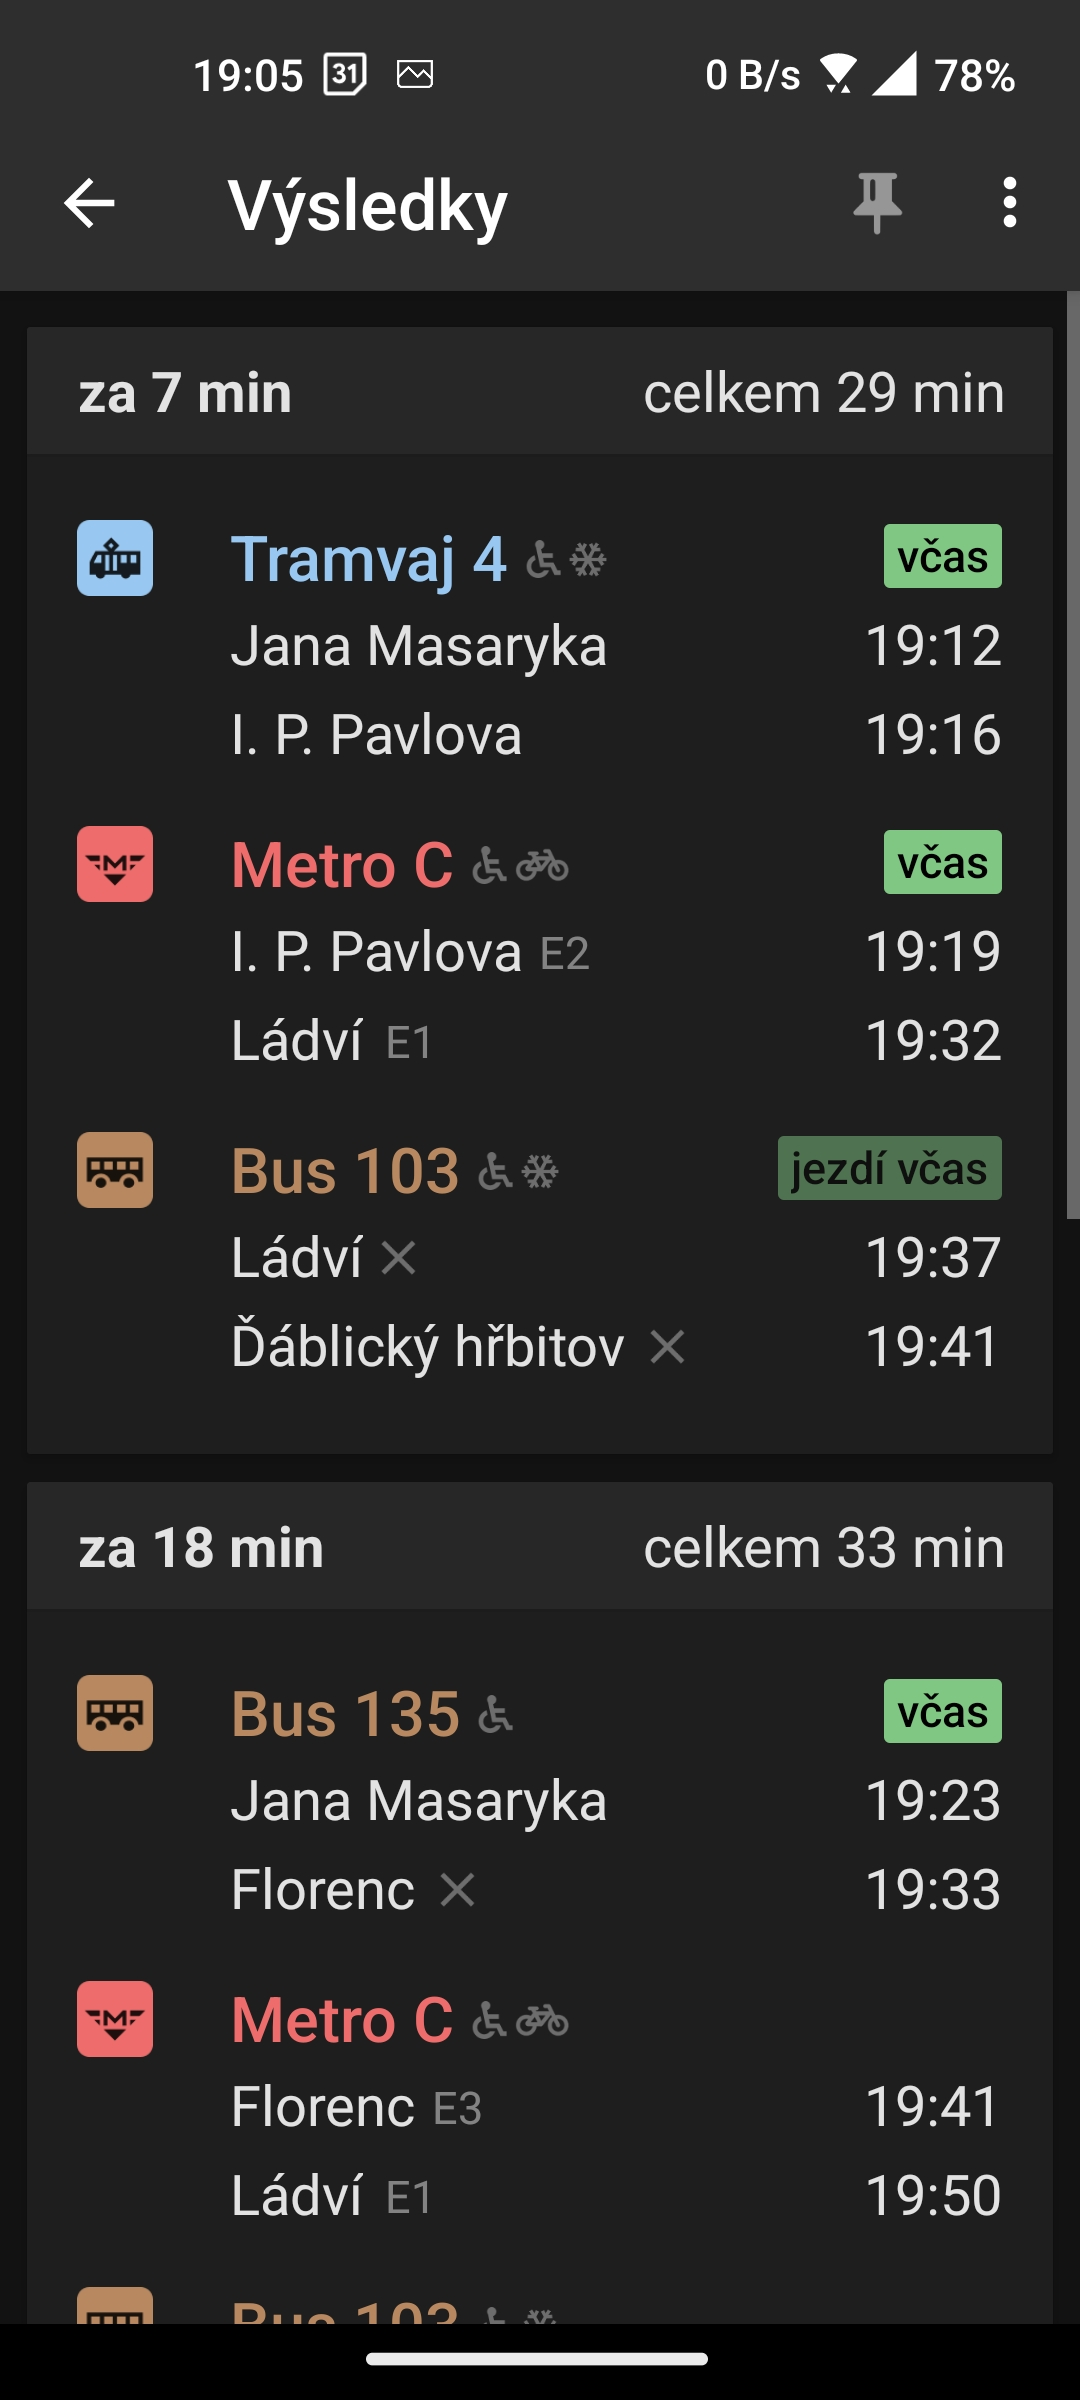
\includegraphics[width=0.45\textwidth]{img/screenshots/pubtran_result.jpg}
    \caption{Result of a connection search in Pubtran}
    \label{fig:pubtran}
\end{figure}

\subsubsection{CG Transit}

The main focus of CG Transit is to provide connection searching while being offline. Additionally, the app also works well online and can use current delay data in the same way as the other apps. It also has some basic configuration options like direct searches, intermediate stops, wheelchair searches, setting global absolute transfer time length and maximum walking time. However, it does not support any more detailed comfort preference settings or setting own walking pace and bikesharing is also not included in the searches. The app uses the more intuitive user interface type similar to IDOS and Pubtran (\cref{fig:cg_transit}).


\begin{figure}[h!]
    \centering
    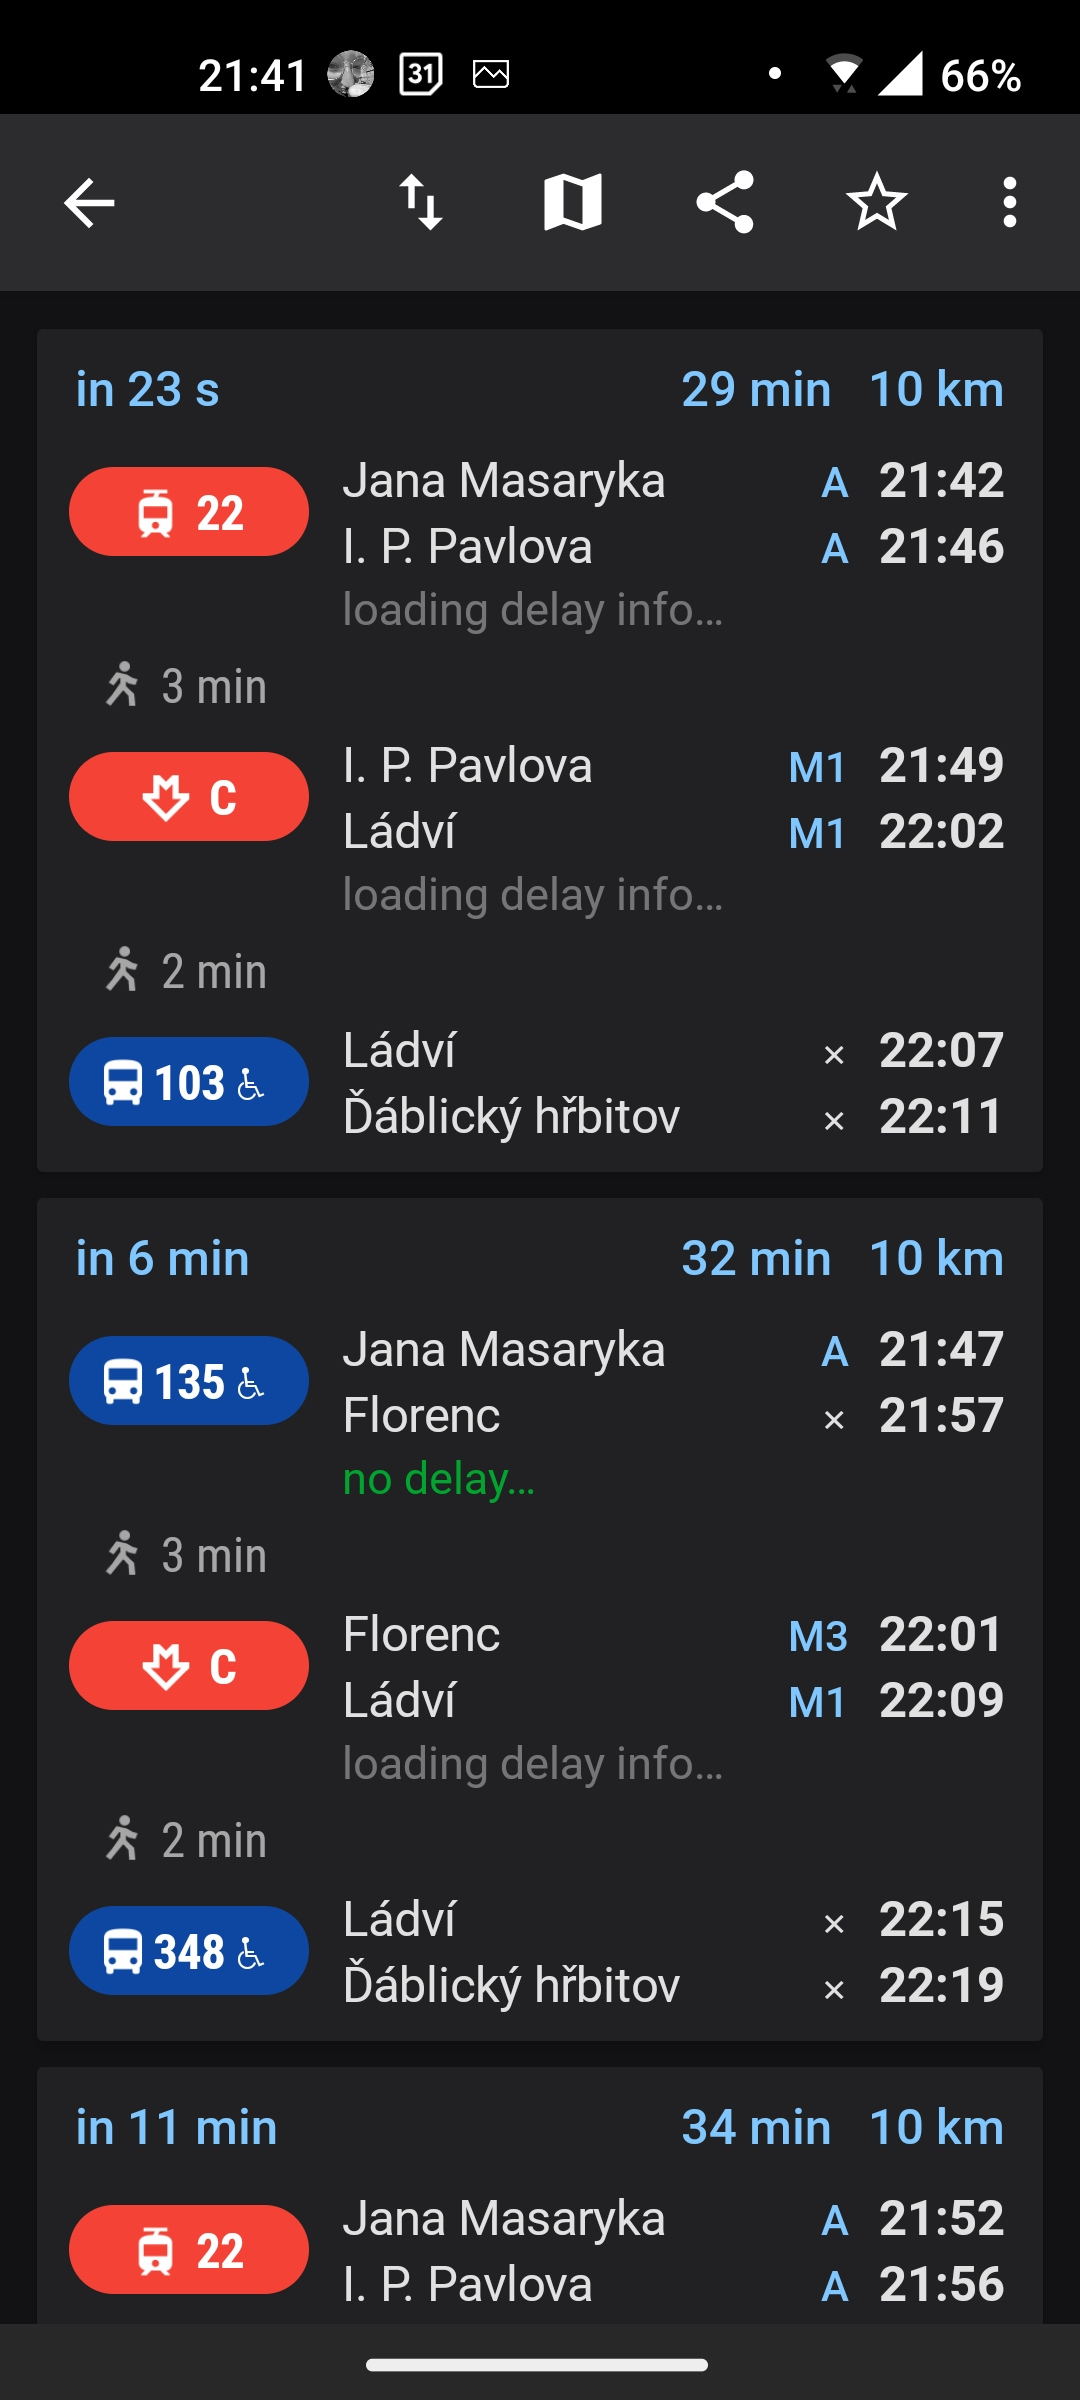
\includegraphics[width=0.45\textwidth]{img/screenshots/cg_transit_result.jpg}
    \caption{Result of a connection search in the CG Transit app}
    \label{fig:cg_transit}
\end{figure}

\subsection{Prague-specific solutions}

\subsubsection{PID Lítačka}

PID Lítačka is the official public transit application developed by the city of Prague. Its main purpose is ticket and transport pass management, but it also includes extensive connection search functionality. The app can be used in 2 modes, classic and advanced. In comparison to the other apps, even in classic mode (which only uses public transport and does not support bikesharing or other modes of transport) the configuration options are much more extensive. There is the option of setting maximum walking distance, maximum transfer count and walking pace (although there are only 3 possible values for Slow, Normal and Fast). It can also search for wheelchair-accessible or low-floor connections. The advanced mode (which at the moment of writing this thesis is in Beta) provides extensive support for other modes of transport, such as own bike or car or shared bikes, scooters, motorcycles, cars and taxis. 

All of this multimodal functionality was added to the app fairly recently and only after the work on this thesis was begun. But, while this has hindered the intent for the subject of this thesis to be the first app supporting bikesharing inclusion in Prague's public transit connection searches, there still remains room for improvement. Specifically, as opposed to the classic mode which displays the results in a very intuitive and clear form similar to that of IDOS and Pubtran (\cref{litacka_classic}), the advanced mode, due to its inclusion of a broad spectre of transport modes, displays the results in a much less intuitive form similar to those of Maps Google and Moovit (\cref{litacka_advanced}). While in this case it doesn't group the resulting connections by their structure (i.e. lines/routes taken) and instead displays the individual connections, it still provides the user with much less information on where the individual connections will take them through. As our app is targeted to audience that already has experience with Prague's public transit system, the users are expected to be able to use their experience to select the percieved best connection out of the presented results. For example, they might know from experience that in a particular section, a line often gets stuck in traffic or gets very crowded, and they can use this information to select other connections from the list of results. In PID Lítačka's advanced mode, this is made much harder by hiding each connection's route information behind a through-click. 


\begin{figure}[h!]
  \begin{subfigure}{.45\textwidth}
  \centering
    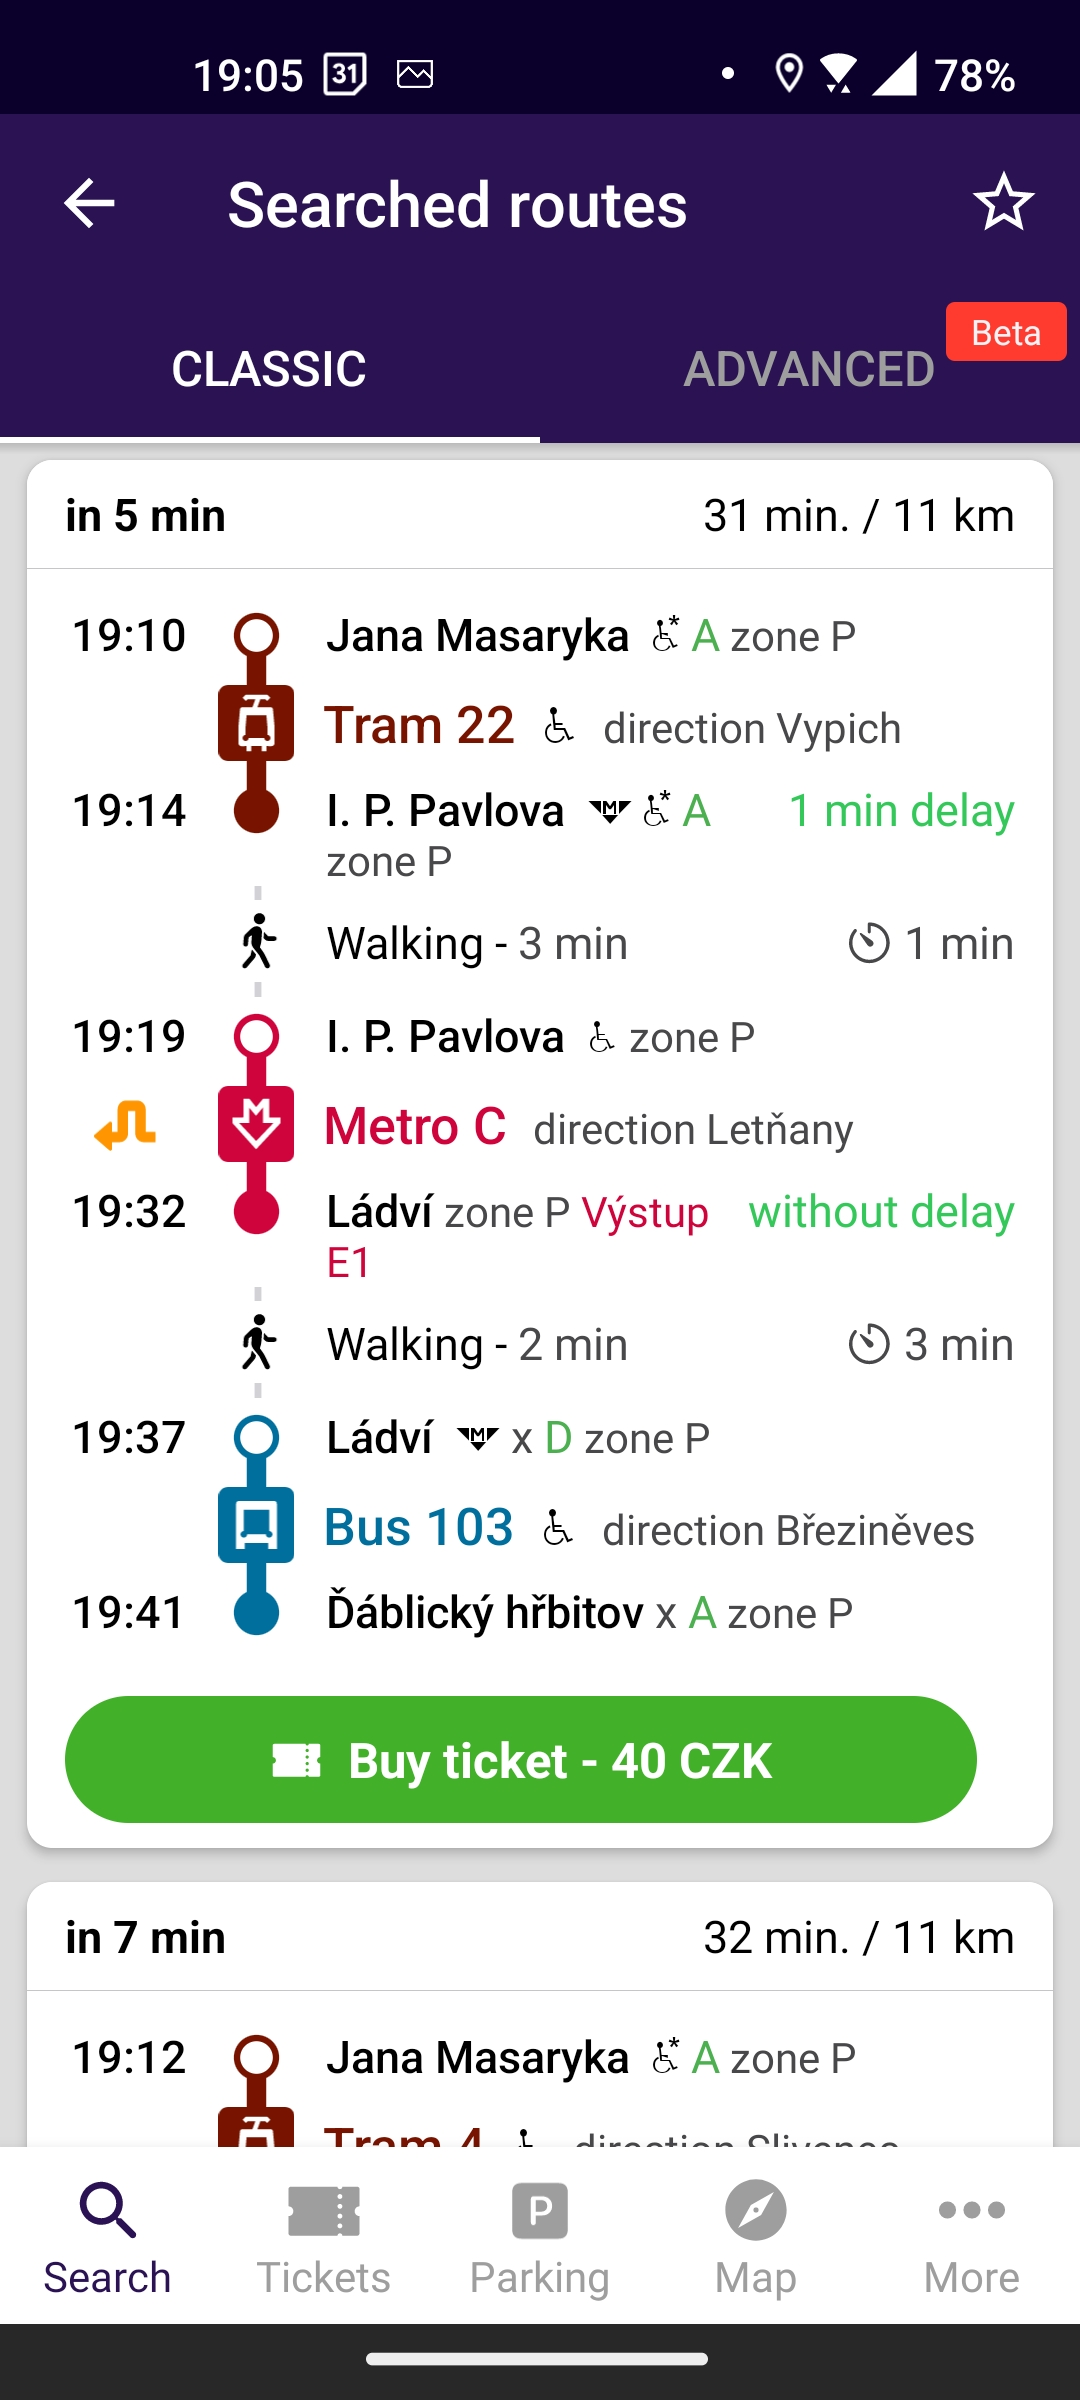
\includegraphics[width=\linewidth]{img/screenshots/pid_litacka_result_simple.jpg}
    \caption{Classic mode}
    \label{litacka_classic}
  \end{subfigure}%
  \hfill
  \begin{subfigure}{.45\textwidth}
  \centering
    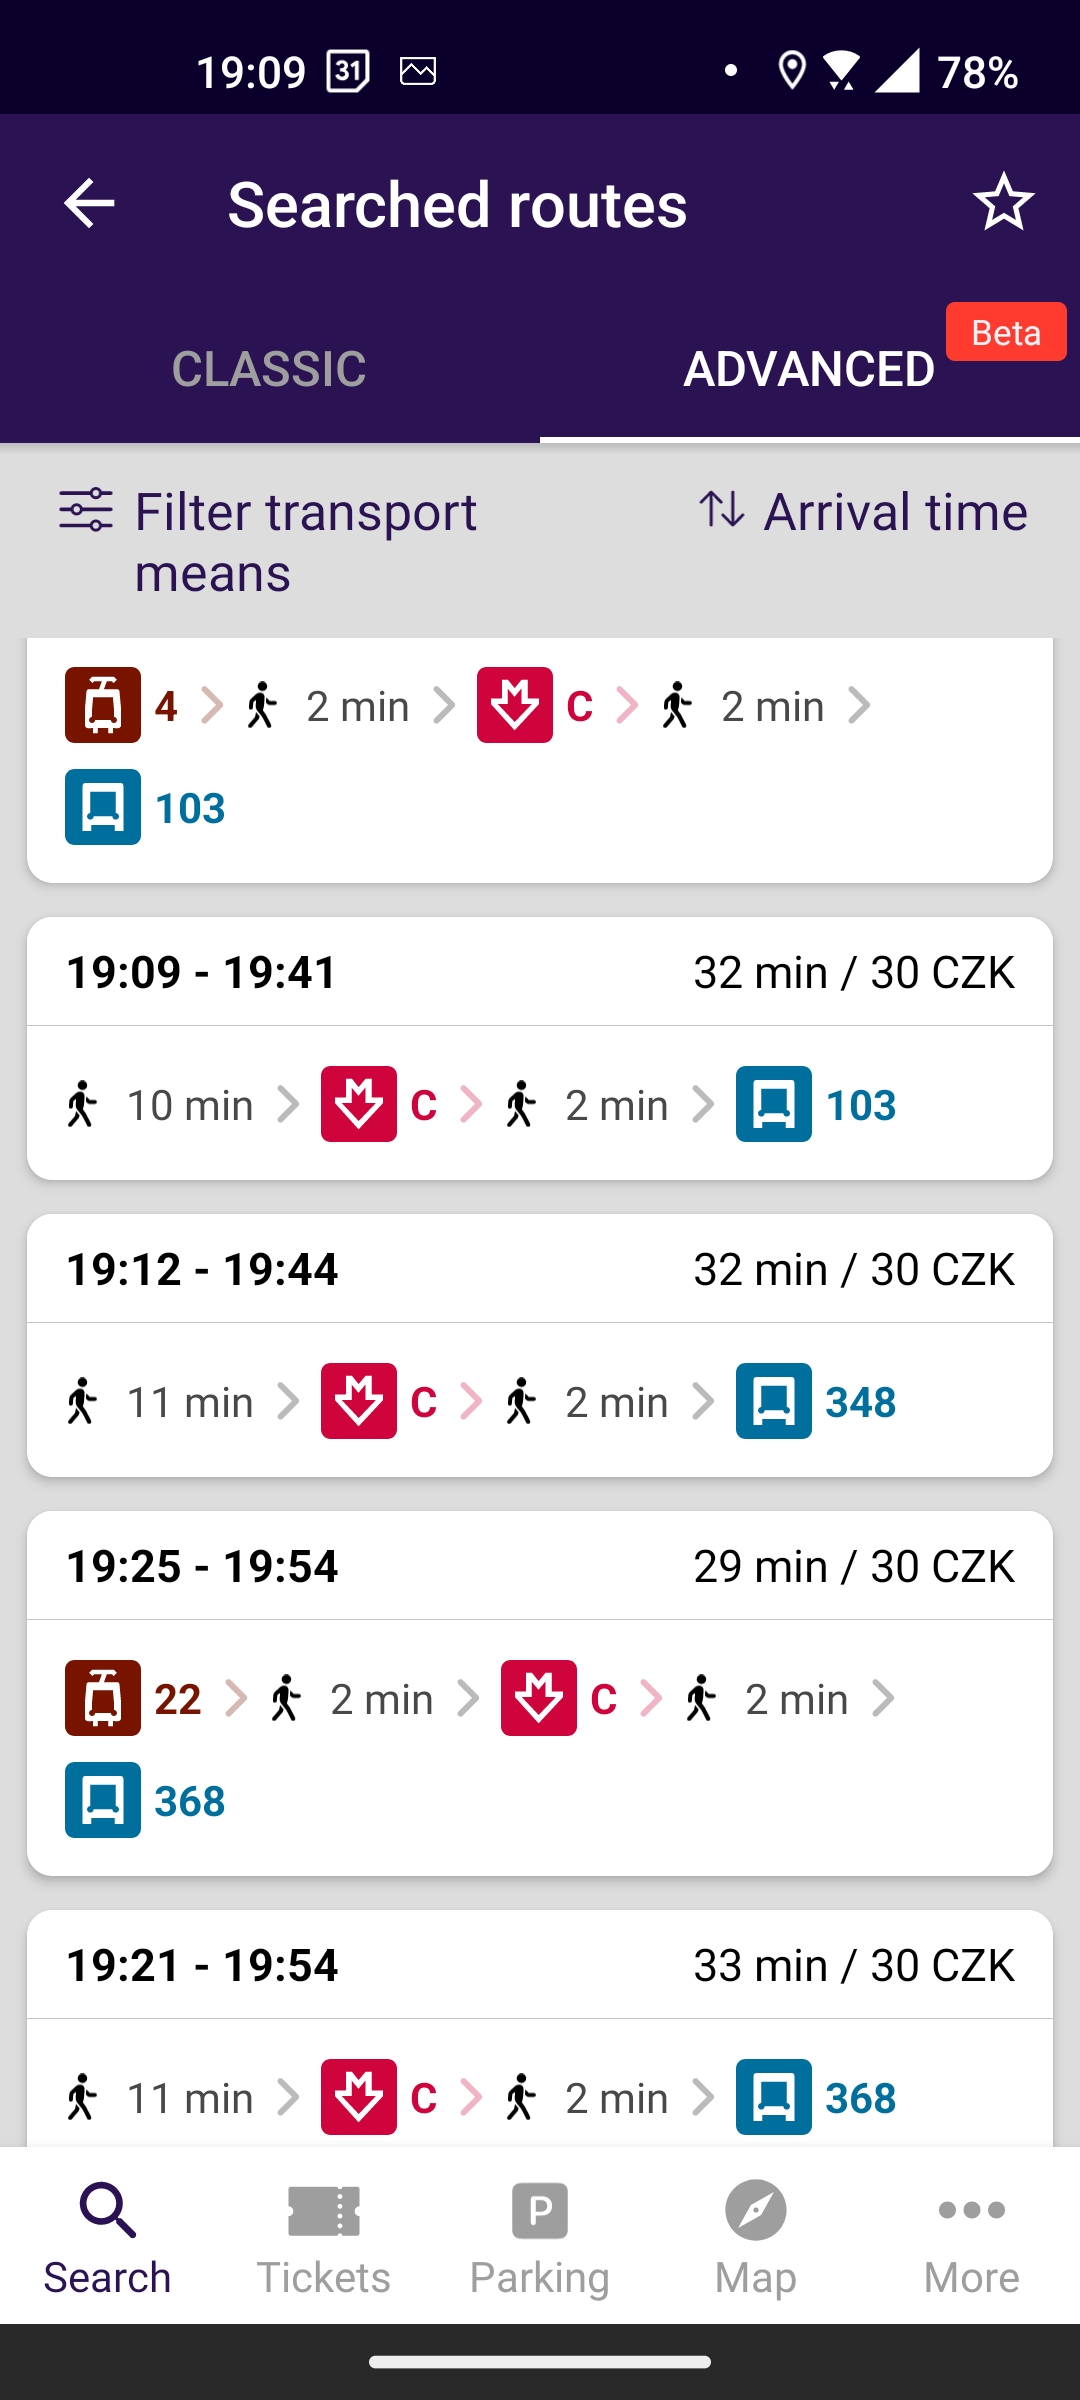
\includegraphics[width=\linewidth]{img/screenshots/pid_litacka_result_extended.jpg}
    \caption{Advanced mode}
    \label{litacka_advanced}
  \end{subfigure}
  \caption{Comparison of search results in PID Lítačka: (a) classic mode and (b) advanced mode}
  \label{litacka}
\end{figure}

\subsection{Other solutions}

There are also other applications we have not included in this overview, such as the official connection search website of Prague's main transport company\footnote{https://spojeni.dpp.cz/} or the Mapy.cz map application from Seznam.cz\footnote{https://mapy.cz/}. However, neither of these solutions exists in the form of a dedicated mobile app. As for most people a mobile application is the go-to way of searching for public transit connections, our goal is to develop such a dedicated application and we thus do not include solutions that only work in the form of a website.

\subsection{Takeaways from the existing solutions}

Although every app we introduced is different, we can observe some larger trends. For example, the applications are divided in terms of the way they display the results. While some apps display only the structure of the connections together with the used lines' names and some even group the resulting connections into groups according to their structure, other apps display each connection separately while showing not only the line names, but also the specific stops at which the individual trips within the connection get boarded and disembarked. While the first approach requires less screen space and can provide a better overview of all the ways one can travel between the two points, the second approach is better suited to the use case our app is designed for, i.e. searching for a connection within one relatively small and dense city. This is because with this approach, the user can have a better overview of what routes are available at the time they need to travel and even more importantly, they can use the additional routing information to select the best option out of the list of results according to their past traveling experience.



Before building our app, we can analyze the features of the existing solutions and select those that contribute most to the goals we set out for our app. As the intended audience for our app are people who use Prague's public transit as a daily tool to get around the city, our goal is to provide them with the option to provide additional input into the connection searches, which will enable them to get better personalized results.

For example, the option to set one's walking (and possibly cycling) pace will improve the relevance of their results, as the durations of transfers and bike trips will better correspond to their habits and preferences, leading to more precise and tailored results. However, even though the user would be able to set their walking pace, there may be situations where they wouldn't be able to walk at their standard pace, such as when transporting heavy luggage or traveling with their older relatives. It would be impractical to assess and change the pace for every connection search. Instead, it would be useful to have the option to set a transfer time buffer value. This could for example be implemented as a simple slider that would be easy and quick to operate before any search that would need it.
The ability to set the maximum length of a transfer would also help to make the results more personalized, as in some situations, the user may prefer not having to perform longer transfers, even if that would mean that the connection would be shorter in time.
While some of the existing apps offer some of these features, none provide all of them in a way that would be usable on a day-to-day basis.

Furthermore, as mentioned above, on two separate occasions, one person may use public transit for two very different things. For instance, when someone is traveling to a work meeting or a school lecture, they will probably want to use the fastest connection. If they are in a big hurry, they might even want to use more transfers than strictly necessary or risk using very short ones, if it means they will be able to get to their destination quicker. On the other end, there may be situations where the same person needs to travel to the airport or railway station with a lot of luggage. In this case, time may not be the limiting factor. Instead, they might want to take the most comfortable route that takes them to their destination using the least possible transfers. Most existing solutions only offer a simple toggle for only searching for direct connections or only setting the absolute maximum number of used trips. Thus, we would like our app to have a more efficient support for specifying the balance between minimizing time and minimizing the number of necessary transfers.

Many of the apps are also able to display current delay information, but do not include it within the connection search algorithm itself. This means that they can suggest connections that are not possible to make due to one of the trips being delayed too much. There is no point in showing such results to the user.

On another note, including bikesharing services within the connection search will lead to users having more options to choose from when traveling through the city. Using shared bikes can often be a faster and/or more pleasant alternative to taking public transit. Also, the city of Prague currently provides bikesharing rides of up to 15 minutes as part of the public transit tickets, so it would also be helpful to be able to limit the maximum length of bike trips to fit in this time frame.

These are just some of the features that some of the mentioned apps provide, and which we would like to include in our application. To provide a better overview, we present the comparison between the features of the existing solutions and those of our application in the table below. The detailed meaning of each feature is described within the app requirements below the table.

\subsection{Comparison of the different solutions}


\overfullrule=0pt
\begin{table}[H]
\centering
\scriptsize % Set base font size to scriptsize
\begin{tabularx}{\textwidth}{ | >{\scriptsize\centering\arraybackslash}m{3.6cm} | >{\tiny\centering\arraybackslash}m{0.8cm} | >{\tiny\centering\arraybackslash}m{0.8cm} | >{\tiny\centering\arraybackslash}X | >{\tiny\centering\arraybackslash}X | >{\tiny\centering\arraybackslash}m{0.8cm} | >{\tiny\centering\arraybackslash}X | >{\tiny\centering\arraybackslash}m{0.8cm} | }
\hline
\textbf{Features\textbackslash Apps} & \textbf{Pubtran} & \textbf{IDOS} & \textbf{Lítačka} & \textbf{Google Maps} & \textbf{CG Transit} & \textbf{Moovit} & \textbf{PragO} \\ \hline
\textbf{Time/Comfort balance setting} & \textcolor{red}{NO}\footnotemark[1] & \textcolor{red}{NO}\footnotemark[1] & \textcolor{orange}{NO}\footnotemark[2] & \textcolor{darkyellow}{PARTLY}\footnotemark[3] & \textcolor{orange}{NO}\footnotemark[2] & \textcolor{darkyellow}{PARTLY}\footnotemark[3] & \textcolor{green}{YES} \\ \hline
\textbf{Adjusting transfer time buffers} & \textcolor{red}{NO} & \textcolor{red}{NO} & \textcolor{green}{YES} & \textcolor{red}{NO} & \textcolor{red}{NO} & \textcolor{red}{NO} & \textcolor{green}{YES} \\ \hline
\textbf{Maximum walking distance} & \textcolor{red}{NO} & \textcolor{red}{NO} & \textcolor{green}{YES}\footnotemark[5] & \textcolor{darkyellow}{PARTLY}\footnotemark[8] & \textcolor{green}{YES}\footnotemark[7] & \textcolor{green}{YES}\footnotemark[7] & \textcolor{green}{YES} \\ \hline
\textbf{Includes bikesharing in searches} & \textcolor{red}{NO} & \textcolor{red}{NO} & \textcolor{green}{YES}\footnotemark[4]\footnotemark[5] & \textcolor{red}{NO} & \textcolor{red}{NO} & \textcolor{red}{NO} & \textcolor{green}{YES} \\ \hline
\textbf{Custom walking/cycling pace} & \textcolor{red}{NO} & \textcolor{red}{NO} & \textcolor{darkyellow}{PARTLY}\footnotemark[6] & \textcolor{red}{NO} & \textcolor{red}{NO} & \textcolor{darkyellow}{PARTLY}\footnotemark[6] & \textcolor{green}{YES} \\ \hline
\textbf{Ability to start search from other nearby stops} & \textcolor{green}{YES} & \textcolor{red}{NO} & \textcolor{green}{YES}\footnotemark[4]\footnotemark[5] & \textcolor{green}{YES} & \textcolor{red}{NO} & \textcolor{green}{YES} & \textcolor{green}{YES} \\ \hline
\textbf{Delay included in planning} & \textcolor{red}{NO} & \textcolor{red}{NO} & \textcolor{red}{NO} & \textcolor{green}{YES} & \textcolor{red}{NO} & UNCLEAR\footnotemark[9] & \textcolor{green}{YES} \\ \hline
\textbf{Metro departure times displayed exactly} & \textcolor{red}{NO} & \textcolor{red}{NO} & \textcolor{red}{NO} & \textcolor{red}{NO} & \textcolor{red}{NO} & \textcolor{red}{NO} & \textcolor{green}{YES} \\ \hline
\textbf{Low data usage} & \textcolor{green}{YES} & \textcolor{green}{YES} & \textcolor{green}{YES} & \textcolor{red}{NO} & \textcolor{green}{YES} & \textcolor{red}{NO} & \textcolor{green}{YES} \\ \hline
\end{tabularx}
\caption{Comparison of features between different apps}
\label{tab:apps_comparison}
\end{table}


\footnotetext[1]{Only provides normal or direct searches}
\footnotetext[2]{Only provides maximum transfer count setting}
\footnotetext[3]{Has no option for absolutely fastest connections, only for "Best Route"}
\footnotetext[4]{Only in Advanced mode, which is currently still in Beta version}
\footnotetext[5]{Feature only introduced after work on this thesis was begun}
\footnotetext[6]{Only 2-3 discrete options (Slow, Normal, (Fast)) - no option to set exact pace}
\footnotetext[7]{Set in minutes, not meters}
\footnotetext[8]{There is only a "Less walking" option}
\footnotetext[9]{The app's UI displays for every trip the first few available options regardless on whether they are reachable by the previous trips of the connection. Due to this, it is unclear whether the delay is included in the planning}


As you can see, most existing apps have very limited possibilities in terms of search personalization options. The only notable exception in this direction is the PID Lítačka app developed by the city of Prague, which added many of the desired features during the last year. Most notably, they recently included bikesharing services within their connection searches, which is a feature that none of the other apps have included yet. However, many of these features were only added after work on our application has commenced, and some features are still missing or implemented only partially. Thus, we set out to implement our own application that would include all of the useful features we mentioned above and would thus be best suited for our target audience. In particular, we set out to fulfill the following functional and qualitative requirements:

\newpage

\section{Requirements}

\begin{enumerate}
\renewcommand{\labelenumi}{\textbf{R\arabic{enumi}}}
\item The user can use the application to find public transit connections in the PID network between two stops of given names, so that they can find the best way to get to their desired destination
\item The user can also find public transit connections using their current location as the starting point, so that they don't need to remember the name of each of the stops near them and don't have to select a single one as the start.
\item The user can search for a connection by providing the earliest possible departure time from the starting point, or the latest acceptable arrival time at the destination point. This is to support both situations where the user is currently at point A and wants to get to point B as soon as possible, and where the user needs to arrive at point B at a certain time and wants to find out at what time they need to set out.
\item The user can set their own walking pace that will be used for calculating transfer times, so that the results better reflect their abilities.
\item The user can adjust this walking pace on a search-to-search basis via a transfer buffer setting, so that they can both allow riskier transfers when they are in a hurry and increase the buffer when they are in a situation where they cannot walk at their normal pace.
\item The user can set the maximum allowed transfer distance, so that they can limit the distance that they would need to walk in situations where they don't want to.
\item The user can set the balance between prioritizing shortest possible time and least possible transfers, so that they can adjust the search to better reflect their current needs and preferences.
\item The user can set the application to include shared bikes in its search algorithm, so that they can see when it might be better to perform a part of the connection on a shared bike instead of taking public transit trips.
\item The user can set the maximum time of a bike trip to 15 minutes, so that the trip can be included as part of their public transit subscription and they do not have to pay for it themselves.
\item The user can set their own cycling pace that will be used for calculating bike trip times, so that the results better reflect their abilities.
\item The user cat set the time it takes them to lock and unlock a shared bike, so that the results better reflect their habits and abilities.
\item If the user sets the source/destination stop name to a specific name, the application will still allow connections starting/ending at other nearby stops. This helps the user in situations where there are multiple different stops nearby served by different routes. It prevents the user from having to run the search for each of the possible source/destination stops separately. 
\item The departure and arrival times are displayed to the user exactly in seconds, especially in the metro. This is to provide the user with exact information on how long they have for a transfer, as in the metro, there is a big difference between a 35 seconds and a 85 seconds long transfer, both of which could be rounded to 1 minute.
\item The application will show multiple different results to the user, so that they can easily select the one that suits them the best.
\item The user can for any used trip in any of the resulting connections display earlier or later alternative trips, so that they know what other alternatives they can take should they not be able to make the one trip the application suggested.
\item For every displayed resulting connection, the application will show the time left until the connection starts. If the connection starts with a walking transfer, it will display both the time left until the user should start walking and the time left until the first trip of the connection leaves. This is so that the user has exact information on when they should leave to make the connection.
\item For every trip of every connection, the application will show its current delay, so that the user can have better overview of the current situation within the city.
\item The application will include and use the delay information during the search and not only add this information to the results. This is to prevent it from presenting connections to the user that are not viable due to the current delay situation.
\item The application needs to keep a relatively low data consumption, to save the user's data consumption. In specific terms, it may not send or receive more than 100kB of data per connection displayed.
\end{enumerate}



\section{Available data}

Our application will need multiple different types of publicly available data to function properly. Firstly, it will need data describing Prague's public transit network with its routes, trips and stops. Secondly, to provide the users with the current delay information and to be able to include it in connection searches, it will need to source this live delay data and to update it frequently. Lastly, it will also require data about the bikesharing networks in Prague to include bikesharing in the searches. To be able to calculate bike routes throughout the city, it will also need some map data of the area covered by the bikesharing providers.

\subsection{Public transit network data}

The transportation agency of the city of Prague publishes the static data describing its public transit network in the GTFS (General Transit Feed Specification) format. This is the industry standard used by transit agencies around the world to provide their data to trip planners, researchers, policy makers, and other third-party apps\cite{gtfs2024}.

The data is available to download from the city website\footnote{http://data.pid.cz/PID\_GTFS.zip} in zip format. The archive contains a total of 20 files, but for our purposes we will only need some of them. In particular, the most important files for our application are \texttt{stops.txt}, \texttt{stop\_times.txt}, \texttt{trips.txt}, \texttt{routes.txt}, \texttt{calendar.txt} and \texttt{calendar\_dates.txt}. In this section, we will take a look at how the data is structured, how the files are linked together and what that means for our application.

\begin{figure}[h!]
    \centering
    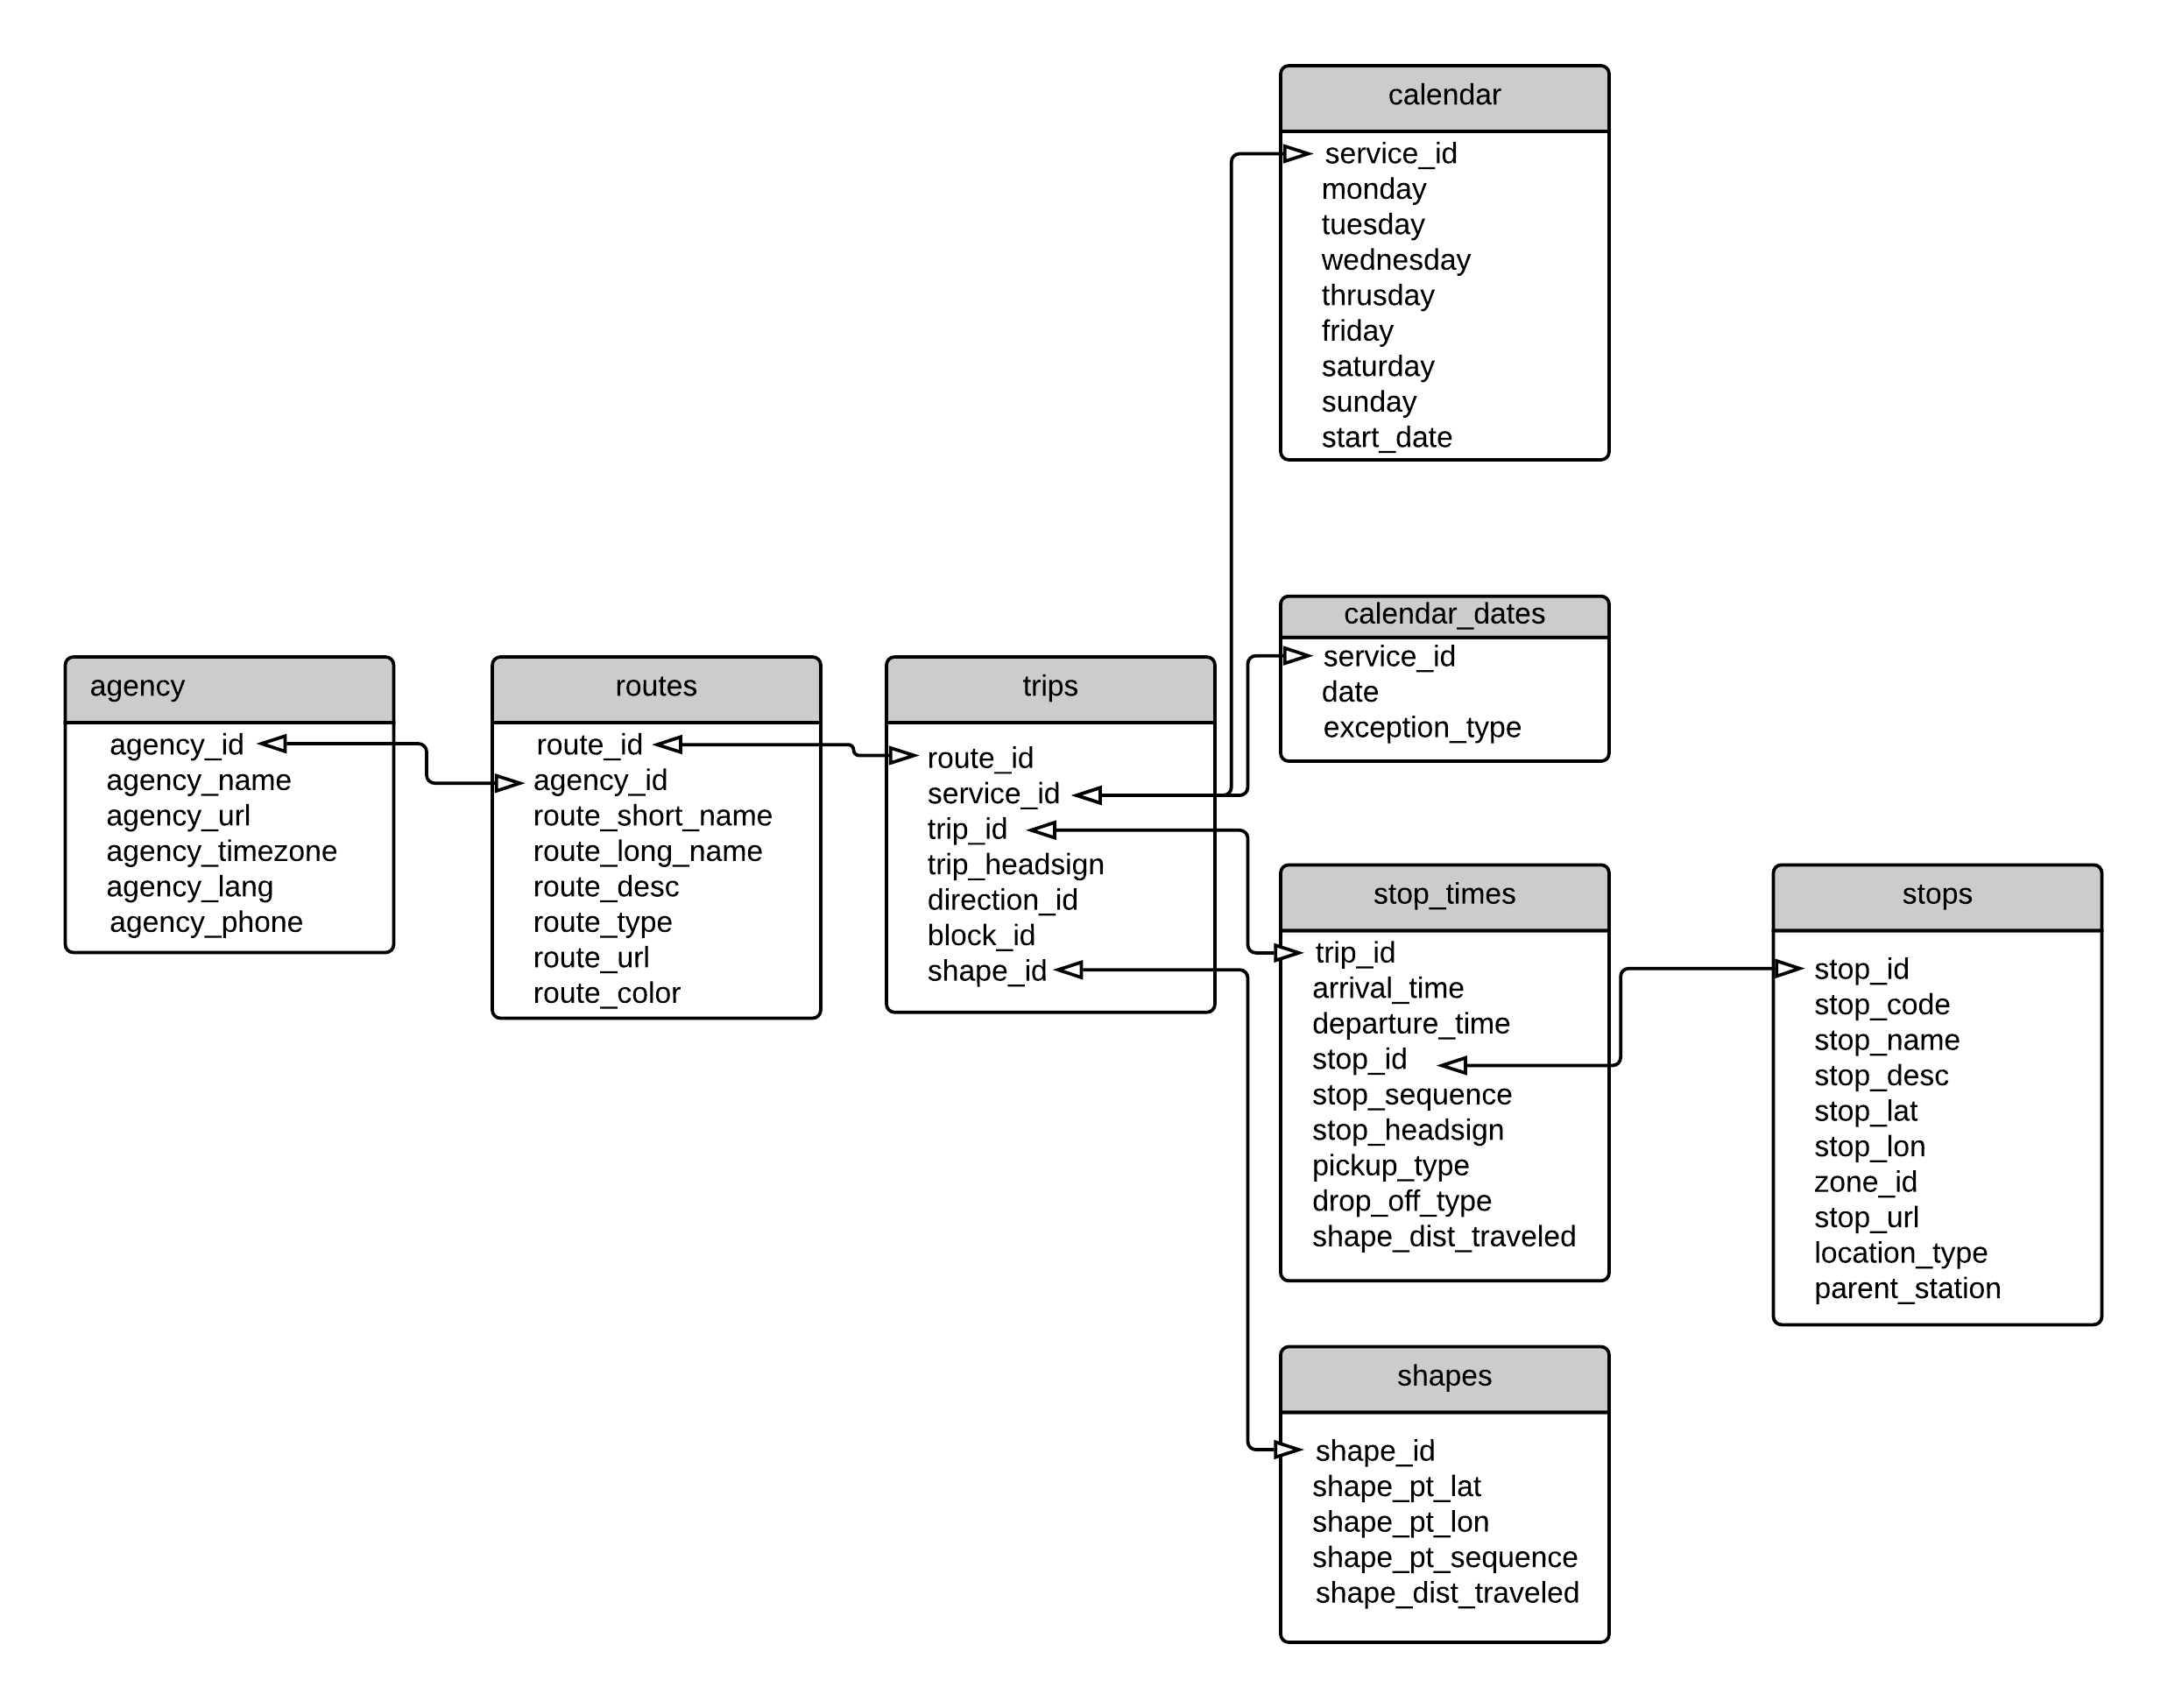
\includegraphics[width=\textwidth]{img/gtfs_scheme.png}
    \caption{GTFS format scheme. Source: Pereira, Andrade and Vieira\cite{pereira2023gtfs}.}
    \label{fig:gtfs_scheme}
\end{figure}

\begin{itemize}
    \item \texttt{stops.txt}
    
    This file contains detailed information about all stops within the network, containing one line per every stop. For our purposes, the most important data within this file are the ids (\textit{stop\_id}), names (\textit{stop\_name}) and the coordinates (\textit{stop\_lat} and \textit{stop\_lon}) of the stops. It also contains information such as what tariff zone the stop is in, an URL of the stop's website or whether the stop is suitable for wheelchair users. However, for our application we will not be using this additional data.

    \item \texttt{routes.txt}

    This file contains information about all the lines within the network. In particular, for every route it holds information about its id (\textit{route\_id}, its short and long names that riders use to identify the route (\textit{route\_short\_name} and \textit{route\_long\_name}, and the type of vehicle that serves the route (\textit{route\_type}). As described earlier, in the context of this thesis, we use the term \texttt{Route} to describe a single variation of a real-world line with its own list of stops. However, one line of the file corresponds to one real-world public transit line, not to one \texttt{Route}. We will construct the individual \texttt{Routes} during the parsing stage by combining the data from this file with the data from the \texttt{trips.txt} and \texttt{stop\_times.txt} files.

    \item \texttt{trips.txt}

    This file contains information about all the trips within the network. Every trip references a single line from the \texttt{routes.txt} file. It also has its own id (\textit{trip\_id} through which a trip is referenced in the \texttt{stop\_times.txt} file. Finally it contains a \textit{service\_id}, which refers to an entry within the \texttt{calendars.txt} and \texttt{calendar\_dates.txt} files. The other information like the trip's headsign will not be used by our application.

    \item \texttt{stop\_times.txt}

    This is typically the largest file in the archive, as it holds most of the useful information about trips and their stop times within the network. It contains a single line per every stop of every trip. The trip is referenced via the \textit{trip\_id} property. The stop is referenced via the \textit{stop\_id} property. It contains both the time of arrival (\textit{arrival\_time}) and departure (\textit{departure\_time}) of the trip at the stop. It also contains the stop's index within the trip's stop list (\textit{stop\_sequence}). The other information will not be necessary for our purposes.

    \item \texttt{calendar.txt}

    As the \texttt{stop\_times.txt} file only contains times and not dates of the trips' stops, this information needs to be present somewhere else. Via the \textit{service\_id} property, each line of this file specifies the dates at which the trip with that \textit{service\_id} is active. It does this by providing start and end dates of the time frame (\textit{start\_date} and \textit{end\_date}) and boolean values specifying on what days of the week between the dates the trip is active (\textit{monday} - \textit{sunday} properties).

    \item \texttt{calendar\_dates.txt}

    This file specifies exceptions to the rules within the \texttt{calendar.txt} file. Every line is once again indexed by a \textit{service\_id} and it contains a \textit{date} and \textit{exception\_type}, which specifies whether this is a positive or negative exception (i.e. whether it has been added or removed for the speciffied date).

    \item Other files

    There are also many additional files with data describing fares, fare zones, guaranteed transfers, metro and train station pathways and trip paths, which our application does not use.
\end{itemize}

In Prague, this data is updated daily between approximately between 4:00 and 4:30\cite{pidopendata}. It's validity is typically around one to two weeks. Thus, our application needs to refresh this data every day to stay up to date.

\subsection{Delay data}

To provide users with current information about delays within the network and to use this data to provide more relevant results, we will need to be able to source this dynamic real-time data periodically from a GTFS Realtime data source. This is again a format designed specifically for this purpose. As opposed to the GTFS Static format described above, this data is not provided in text form. Instead, it is available as a protocol buffer\cite{gtfs2024}, which is Google's language-neutral, platform-neutral and extensible mechanizm for serializing structured data\cite{protobuf2024}. This data is available through an official API of the city of Prague\footnote{https://api.golemio.cz/pid/docs/openapi/}. A total of 3 files are provided - \texttt{trip\_updates.pb}, \texttt{vehicle\_positions.pb} and \texttt{alerts.pb}, which contain information on current delays, real-time positions of public transit vehicles and current disruptions within the network respectively. Prague also provides a \texttt{pid\_feed.pb} file, which is just the first 2 files combined into one feed.

As we are only interested in the time values of delays within the network and do not need information on exact GPS coordinates of every trip, the only file relevant to our application is the \texttt{trip\_updates.pb} file. In particular, it contains \textit{stop\_time\_updates} for every active trip, which specify the actual or expected stop times at the trip's stops. It also contains an experimental \textit{delay} field specifying the length of the current delay compared to the scheduled time. This is all the information we will need to implement delay handling within our application, and thus we won't be using the other provided data fields.

\subsection{Bikesharing data}

While the city of Prague has direct access to data about the bikesharing systems of the Rekola and Nextbike companies thanks to their contract with them, this contract prevents them from publishing this data directly through their API. Unfortunately, there is no way to publically access this data of the Rekola company, which prevents us from including it's bikes within our searches. Fortunately however, the Nextbike company publishes the data about all of their bike systems around Europe, so we can access the Prague-specific data from this API. Thanks to this, we only need to use the network id of Prague to access the data in GBFS format from their website\footnote{https://gbfs.nextbike.net/maps/gbfs/v2/nextbike\_tg/cs/<FILE\_NAME>}.

While the GTFS format standardizes data about public transit networks, GBFS (General Bikeshare Feed Specification) does the same for bikesharing providers who want to publish standardized data about their networks. As opposed to GTFS, which mostly uses a CSV-like format, the GBFS files use JSON\cite{gbfs2024}. Our application only will be using 2 of the provided files:

\begin{itemize}
    \item \texttt{station\_information.json}

    This file contains static information about the bike stations within the network. In particular, for every station there is a \textit{station\_id}, a \textit{name}, a location (\textit{lat} and \textit{lon}). There also is a lot of additional information, such as the type of the station, its opening hours or rental methods, which we will not be using, as this information is the same for all of Nextbike's stations within Prague. The stations also have a \textit{capacity} property, however, this does not seem relevant in any way in Prague, as this capacity is not enforced in any way and can be exceeded freely, so we will not be using this value either.

    \item \texttt{station\_status.json}

    The main information contained within this file is the number of free bikes available at each station. Again, for our purposes we will only be using the \textit{station\_id} and \textit{num\_vehicles\_available} properties, as the other information is irrelevant in our setting.
\end{itemize}



\subsection{Map data}

As part of our application, we will need to implement bike routing within the city. In contrast to the public transit trips, the routes of which are directly specified within the data itself, for bikesharing services, we only have the list of stations and need to find the paths between them ourselves. One way to solve this problem would be to use an external routing API, such as the one from Mapy.cz, which provides this exact functionality\cite{mapyczapi}. However, such API's are typically paid, which would be problematic for calculating a large number of connections. Furthermore, as our application will not show the trips on a map, it only needs information about the trip's length and duration and not its exact path. Paying for getting the exact best route when we will not need it seems wasteful, and thus we decided to use our own routing.

As implementing the whole routing functionality would be way out of scope for this project, we have used a library for this purpose, which will be described in detail in following chapters. This library, like all other alternatives that provide this routing functionality, requires map data to function. In particular, it uses the Open Street Maps project and its maps. These maps are provided free of charge for every region in the world. As the maps do not provide smaller granularity within the Czech Republic than the whole country, we will use this country-wide map file from the website\footnote{https://download.geofabrik.de/europe/czech-republic.html}. This file has the \textt{.pbf} format. In our application, we then parse this file into a new \texttt{.routerdb} file, which is a proprietary format that the library uses to provide efficient routing. As the details on the inner implementation of these files are irrelevant for our project, as we do not directly manipulate them, we will not include them within this document.

\subsection{Data that is currently not available}

As stated above, the bikesharing company Rekola does not publish its data and we thus cannot include their bikes within our searches.

The other type of data that would be helpful, but doesn't yet exist, would be some kind of data on the possible transfers within Prague's public transit network. Currently, there is no such data available, and so every application needs to calculate its transfers itself. Theoretically, the same map data and library that we use for bike routing could be used for this purpose, but this would be extremely inefficient due to the large number of stops within the network. Because of this, in our application, we only use the direct line distances between every pair of stops to calculate what transfers are possible and how long they are. A data set containing the distances between all stops where a transfer is possible would be very useful for connection planning apps, as it would make the results more relevant and exact.



